%%%%%%%%%%%%%%%%%%%%%%%%%%%%%%%%%%%%%%%%%%%%%%%%%%%%%%%%%%%%%%%%%%%%%%%%%%%%%%
%%
%% This file is part of the ASTERICS Framework. 
%%
%% (C) 2019 Hochschule Augsburg, University of Applied Sciences
%% Efficient Embedded Systems Group
%%
%% Author(s): Philip Manke <philip.manke@hs-augsburg.de>
%%
%%%%%%%%%%%%%%%%%%%%%%%%%%%%%%%%%%%%%%%%%%%%%%%%%%%%%%%%%%%%%%%%%%%%%%%%%%%%%%



\section{Automatics - The Chain Generator} \label{ch:06-02-tools-generator}

\secauthor{Philip Manke}

This chapter introduces and describes the functionality of Automatics, the \asterics processing chain generator.

Automatics uses a short, user-editable Python script to generate, several possible output products, including hardware source files, software source files, a functional IP-Core (currently only in the Vivado-format) and an SVG graph.

Section \ref{sec:06-02-user_guide} gives a brief overview of the functionality of Automatics and section \ref{sec:06-02-interactive} briefly explains the module browsers available with Automatics which we recommend to use while developing \asterics chains.
Sections \ref{sec:06-02-default}, \ref{sec:06-02-new_modules}, \ref{sec:06-02-interactive}, \ref{sec:06-02-quirks} and partly \ref{sec:06-02-config_methods}, provide more details for a deeper understanding of Automatics.
Information about developing 2D Window Pipeline systems using Automatics is provided in section \ref{sec:06-02-2dpipe_general}.
The steps required to add and use your own hardware modules with Automatics are described in section \ref{sec:06-02-new_modules}.
Section \ref{sec:06-02-objects} provides additional information about the internal structure of Automatics and more advanced configuration methods, which may be of interest when developing complex \asterics chains, when investigating errors reported by Automatics and especially when developing Automatics itself.

\subsection{User Guide}
\label{sec:06-02-user_guide}

This section gives a summarized explanation of how to generate an \asterics system using Automatics.

This guide will walk through the generation of a demo system as included with \asterics.
All necessary steps are explained, with a focus on steps involving Automatics.


\subsubsection{Step 0: Prerequisites}

\begin{itemize}
\item An \asterics installation: Check Section \ref{sec:02-installation}
\item Python 3.5 or a higher version
\item (mostly optional) Basic knowledge of VHDL syntax
\item (optional) GraphViz tool (\texttt{>= 2.38}) and Python module \texttt{graphviz} (\texttt{>= 0.8}) for visualization 
\item (optional) A synthesis tool for your type of FPGA
\item (optional) A hardware target - we suggest the ZyboBoard with an OmniiVision OV7670 camera module 
\item For CNN systems: Python package \texttt{numpy}
\end{itemize}

\infobox{For correct operation, your system needs to use a UTF-8 based locale.}

\subsubsection{Step 1: Setting up the Work Environment}

\begin{enumerate}
\item Locate your ASTERICS installation and move there using the command line.
\begin{lstlisting}[style=shell]
 > cd <path to asterics>
\end{lstlisting}
\item If Vivado is installed on the system and you want to use it for this guide, source the Vivado settings file at this time.
In the Xilinx installation directory, it should be located under \texttt{"Xilinx/Vivado/<version>/settings64.sh"}.
ASTERICS requires the environment variable \texttt{XILINX\_VIVADO} to be set to start Vivado automatically.
\begin{lstlisting}[style=shell]
 > source <installation path>/Xilinx/Vivado/<version>/settings64.sh
\end{lstlisting}
\item Source or run the script \texttt{"settings.sh"} in the root of the ASTERICS installation.
\begin{lstlisting}[style=shell]
 > source settings.sh
\end{lstlisting}
\item Navigate to the folder \texttt{"<asterics>/systems/"} and copy the folder \texttt{"as\_refdesign\_zynq"} to the location where you want to generate the system.
\begin{lstlisting}[style=shell]
 > cd systems
 > cp -a as_refdesign_zynq <target path>
\end{lstlisting}
\end{enumerate}


\subsubsection{Step 2: Modifying the Chain Description (optional)}

Move into the directory \lsthdlinline{as_refdesign_zynq/asterics/image_differencing/}.
In this folder the chain description script, \lsthdlinline{asterics-gen.py}, is located, containing the method calls in Python syntax that describe the makeup of the \asterics chain / system.

An \asterics chain is comprised of modules that execute specific image processing and general data management tasks. Modules are added to the chain using the \lstapyinline{chain.add_module()} method.
This method takes two parameters: \lstapyinline{chain.add_module(<module name>, <custom name>)}.
The \lstapyinline{<module name>} is identical to the name of the VHDL entity of the module's toplevel VHDL file.
The optional \lstapyinline{<custom name>} parameter can be anything, as long as there are no duplicates in a system.
This name is used to associate signal, port and address names to the module.
To find out which modules are available, the interactive Automatics environment or GUI can be used by calling \texttt{as-module-browser-cli} or \texttt{as-module-browser} on the console, after sourcing the \asterics settings file.
Alternatively the \texttt{modules} folder of the \asterics installation can be manually browsed, as the names of the contained folders are usually identical to the VHDL entities (there are exceptions and folders containing more than one module).

The \lstapyinline{add\_module()} method returns a reference to the newly created module object, which should be assign to a new variable.
With this object, a \lstapyinline{connect()} method can be used to connect two modules to each other. Several objects within Automatics provide \lstapyinline{connect()} methods:
\begin{itemize}
\setlength\itemsep{0.3em}
\item Module objects: \lstapyinline{<source module>.connect(<target>)}\\Example: \lstapyinline{camera.connect(collect)}
\item Interface objects: \lstapyinline{<source>.connect(<target>)}\\Example: \lstapyinline{splitter.get("1").connect(invert)}
\item Port objects: \lstapyinline{<source>.connect(<target>)}\\Example: \lstapyinline{camera.get_port("vcomplete_out").connect(collect)}
\item The \lstapyinline{chain} object: \lstapyinline{chain.connect(<source>, <target>)}\\Example: \lstapyinline{chain.connect(camera, collect)}
\end{itemize}

The target used in a \lstapyinline{connect()} method does not need to be of the same "type" as the source.
Note: Before using an object as a target in a \lstapyinline{connect()} method, it must have been created and added to the chain using the \lstapyinline{chain.add_module()} method.

Using the \lstapyinline{module.get(<name>, <direction>)} method or the more specific \lstapyinline{module.get_interface(<interface name>)} and \lstapyinline{module.get_port(<port name>)} methods, \lstapyinline{connect()} methods can be used to connect individual ports and interfaces.
Additionally, the module objects returned by the \lstapyinline{chain.add_module()} method can be used to configure many aspects of the modules and how they are integrated into the \asterics system.
For a reference of the available methods, refer to section \ref{sec:06-02-config_methods}.

Here are two examples for system definition functions:

\medskip

\textit{Example 1 (Listing \ref{Code:06-02-define_invert}):} A simple processing chain, reading an image from an Omniivision camera in grayscale, inverting all pixels and writing the result into memory.
This system uses just four hardware modules.

\begin{lstlisting}[style=AutomaticsPython, label=Code:06-02-define_invert, caption=Definition of a simple invert system]

# as_invert demo system:
# (HW ->) camera -> invert -> collect -> writer (-> RAM)

# Setup
import asterics
chain = asterics.new_chain()

# -------- Module instantiations ------------------------
camera = chain.add_module("as_sensor_ov7670", "camera0")
invert = chain.add_module("as_invert")
collect = chain.add_module("as_collect")
writer = chain.add_module("as_memwriter", "writer")

# -------- Module configurations ------------------------
camera.add_iic_master("XILINX_PL_IIC")
writer.set_generic_value("MEMORY_DATA_WIDTH", 32)
writer.set_generic_value("DIN_WIDTH", 32)

# -------- Module connections ---------------------------
camera.connect(invert)
invert.connect(collect)
collect.connect(writer)
\end{lstlisting}

\bigskip

\textit{Example 2 (Listing \ref{Code:06-02-define_diff}):} A processing chain with multiple branches calculating the differences in pixel values of two subsequent video frames.
This is the description for the reference design used in this guide (\texttt{as\_refdesign\_zynq}).
\medskip

\begin{lstlisting}[style=AutomaticsPython, label=Code:06-02-define_diff, caption=Definition of a system calculating pixel value differences over time]
# Difference demo system:
# (HW ->) camera -+-> collect0 -> writer0 (-> RAM)
#                 \-------------->\ 
# (RAM ->) reader -> disperse -> sync => pixel_diff -> ... 
#              ... -> collect1 -> writer1 (-> RAM)

# Setup
import asterics
chain = asterics.new_chain()

# -------- Module instantiations ------------------------
# Camera
camera = chain.add_module("as_sensor_ov7670", "camera")
camera.add_iic_master("XILINX_PL_IIC")
# Reader
reader = chain.add_module("as_memreader")
# Disperse
disperse = chain.add_module("as_disperse")
# Stream Sync
sync = chain.add_module("as_stream_sync")
sync.set_generic_value("BUFF_DEPTH", 1024)
# Pixel Diff
diff = chain.add_module("as_pixel_diff")
# Collect modules
collect0 = chain.add_module("as_collect", "collect0")
collect1 = chain.add_module("as_collect", "collect1")
# Writer 0
writer0 = chain.add_module("as_memwriter", "writer0")
writer0.set_generic("MEMORY_DATA_WIDTH", 32)
writer0.set_generic("DIN_WIDTH", 32)
# Writer 1
writer1 = chain.add_module("as_memwriter", "writer1")
writer1.set_generic("MEMORY_DATA_WIDTH", 32)
writer1.set_generic("DIN_WIDTH", 32)

# -------- Module connections ---------------------------
# original image path:
camera.connect(collect1)
collect1.connect(writer1)

# previous image read path:
reader.connect(disperse)

# sync image pixels, diff and write back the result:
disperse.connect(sync.get("0", "in"))
camera.connect(sync.get("1", "in"))
sync.get("0", "out").connect(diff.get("0", "in"))
sync.get("1", "out").connect(diff.get("1", "in"))
diff.connect(collect0)
collect0.connect(writer0)
\end{lstlisting}

\bigskip

Below, a brief list of the most important commands for use in the chain description script is included, for quick reference.
A full list of commands provided for use in the chain description script is available in section \ref{sec:06-02-config_methods}.

\begin{itemize}
\item \lstapyinline{chain.add_module(<entity name>, <custom name>)}: Add the module with \lstapyinline{<entity name>} to the system and optionally name it \lstapyinline{<custom name>}.
This method returns the added module as an object which should be assigned to a variable, for example:
\lstapyinline{inverter = chain.add_module("as_invert", "myinverter")}
\item \lstapyinline{module0.connect(module1)}: Create connections between any compatible interfaces and ports from \lstapyinline{module0} to \lstapyinline{module1}.
The \lstapyinline{connect()} method can be used from any module, interface and port to any module interface and port, for example:\\
\lstapyinline{module0.get_port("data").connect(module1)}\\
\lstapyinline{module0.get_interface("0").connect(module1.get_interface("in"))}\\
\lstapyinline{module0.connect(module1.get("image"))}
\item \lstapyinline{module.make_port_external(<port name>)}: Automatics will pull this port to toplevel, so it faces the outside of the generated hardware
\item \lstapyinline{module.make_interface_external(<interface name>)}: Same functionality as \lstapyinline{make_port_external} but for an entire interface.
\item \lstapyinline{module.set_port_fixed_value(<port name>, <value>)}: Set this port to the specified value. Note: Automatics directly writes the parameter \lstapyinline{<value>} into VHDL code, so its value must not violate VHDL syntax.
\item \lstapyinline{module.set_generic_value(<generic name>, <value>)}: Same as the above command, but for VHDL Generics instead of ports. Generics are used to configure the functionality and properties of hardware modules.
\item \lstapyinline{module.make_generic_external(<generic name>)}: Automatics will propagate the generic to the toplevel - the interface of the generated hardware / IP-Core.
This allows to adjust the value of the generic using the synthesis tool.
\item \lstapyinline{module.get_interface(<interface name>, <direction>)}: Return the interface with the name \lstapyinline{<interface name>} of \lstapyinline{module}. Use in conjunction with a \lstapyinline{connect()} method to connect specific interfaces.
\item \lstapyinline{module.get_port(<port name>)}: Return the port \lstapyinline{<port name>} of \lstapyinline{module}. Use in conjunction with a \lstapyinline{connect()} method to connect specific ports.
\item \lstapyinline{module.get(<name>, <direction>)}: Return the interface or port \lstapyinline{<name>} of \lstapyinline{module}. This convenience method first calls \lstapyinline{get_interface()} and, if no interface \lstapyinline{<name>} was found, then calls \lstapyinline{get_port()}. Note that the parameter \lstapyinline{<direction>} only applies to interfaces. This method may be used as a shorthand for either of the more explicit methods.
\end{itemize}

You may edit the system described in \texttt{asterics-gen.py}, note however, that the supplied software in the file \texttt{asterics-demo.c} might not be compatible with any changes to the systems hardware.
We suggest to first generate the system without having made changes to verify that the generator works as expected on your system.
Afterwards a copy of the script and software - or the entire project - may be used as a basis for your own ideas.


\subsubsection{Step 3: Generating Output Products}

In the root of the demo system \texttt{as\_refdesign\_zynq} a Makefile is provided.
The Makefile can automatically generate the entire system, implement it using Vivado, compile the software and flash it to hardware.
If you have a ZyboBoard and OV7670 camera, you can obtain a functional system by connecting the board to you computer and calling 
\begin{lstlisting}[style=shell]
 > make
\end{lstlisting}
on the commandline, provided your Vivado installation already includes the board files for the ZyboBoard.

Optionally, with Vivado installed the bitfile can be generated and the software compiled by running 
\begin{lstlisting}[style=shell]
 > make asterics_vivado_cores && make build_system
\end{lstlisting}
on the commandline.
The output will be generated to the folders \texttt{hardware}, \texttt{vivado\_cores} and \texttt{software}.

The system generator can also be run alone by executing the \texttt{asterics-gen.py} script using Python 3.
In the commandline run:
\begin{lstlisting}[style=shell]
 > python3 asterics/image_differencing/asterics-gen.py vivado vivado_cores
\end{lstlisting}
or using the Makefile:
\begin{lstlisting}[style=shell]
 > make asterics_vivado_cores
\end{lstlisting}
This will generate the ASTERICS IP-Core to \texttt{vivado\_cores}.

If Vivado is not installed, the IP-Core packaging step can be skipped to just obtain the source files, both hardware and software for the ASTERICS system by running:
\begin{lstlisting}[style=shell]
 > python3 asterics/image_differencing/asterics-gen.py core asterics_core
\end{lstlisting}
or using the Makefile:
\begin{lstlisting}[style=shell]
 > make asterics_core
\end{lstlisting}
The output will be generated to \texttt{asterics\_core}.\\
For all generator targets of this demo system, an SVG graph of the internal processing chain will be generated to the root folder of the system with the name \texttt{asterics\_system\_graph.svg}.
In the Automatics script, this is achieved by the following command:
\begin{lstlisting}[style=AutomaticsPython]
chain.write_system_graph()
\end{lstlisting}

For more information on this demo system, refer to section \ref{sec:09-01-as_refdesign_zybo}.\\

For future systems, consider copying the script \texttt{asterics-gen.py} or the more generic script in  \lsthdlinline{<asterics>/tools/as-automatics/user_script.py} to use as a template.


\subsection{\asterics Module Browser}
\label{sec:06-02-interactive}

\subsubsection{Command Line Interface}

The command line interface (CLI) of Automatics provides a basic \asterics module browser.
This allows you list the available modules in \asterics, inspect modules and issue Automatics methods calls in a command line environment.
Furthermore, new module repositories can be imported, including your own modules, which can be helpful to make sure that Automatics correctly analyzed your modules.


To start the CLI module browser the \asterics settings file has to be sourced first on the command line:
\begin{lstlisting}[style=shell]
 > source <asterics installation path>/settings.sh
\end{lstlisting}

Then it can be started using:
\begin{lstlisting}[style=shell]
 > as-module-browser-cli
\end{lstlisting}

Now Automatics is loaded and the modules present in the \asterics installation path are automatically imported.
The functions available for exploring the modules and adding new repositories can be listed with the command \lstapyinline{as_help()}.
Further details about the functions can be shown using \lstapyinline{<function name>?}.
For example:
\lstapyinline{module_detail?}

\subsubsection*{Prerequisites:}

\begin{itemize}
\item An \asterics installation
\item Python (version \texttt{>= 3.5}) 
\item Python package \texttt{ipython} (version \texttt{>= 2.4})
\end{itemize}

\subsubsection{Graphical User Interface}
\label{sec:06-02-gui}

\infobox{Note: The module browser GUI is deprecated and will be removed in future version of \asterics.}

The graphical user interface (GUI) for the \asterics module browser provides a more convenient way to see available modules and to get a quick overview of their interfaces and configuration options.
It provides mostly the same functionality as the command line interface in GUI form.

Currently, two GUIs exist:

\begin{itemize}
\item The newer, more feature-rich \asterics GUI, detailed in Chapter \ref{ch:06-05-tools-gui},
\item and the legacy module browser GUI, described here.
\end{itemize}


To start the legacy module browser GUI, just as with the CLI module browser, the \asterics settings file has to be sourced first, using the command line:
\begin{lstlisting}[style=shell]
 > source <asterics installation path>/settings.sh
\end{lstlisting}

Then the GUI can be started using:
\begin{lstlisting}[style=shell]
 > as-module-browser
\end{lstlisting}

\subsubsection*{Prerequisites:}

\begin{itemize}
\item An \asterics installation
\item Python (version \texttt{>= 3.5}) 
\item QT5 (version \texttt{>= 5.5})
\item The PyQt5 GUI library: \texttt{pyqt5} (version \texttt{>= 5.14})
\end{itemize}


\subsection{Default Behaviour}
\label{sec:06-02-default}

This section briefly explains the default behaviour of Automatics when handling Generics, Interfaces and Ports of the modules you add to a new ASTERICS system.

\textit{Generics} that are left unconfigured will use the default value which is usually present in the VHDL code.
If no default value is available, it will be left blank, causing an error during synthesis.
Therefore, you should check which default values are set for each generic, using the \lstapyinline{module_detail()} function in the interactive mode, the GUI or directly in the VHDL source code, described in section \ref{sec:06-02-interactive}.
Alternatively, \lstapyinline{module.make_generic_external()} can be used to enable editing of the Generic value using the synthesis tool or set a fixed value using \lstapyinline{module.set_generic_value()}.

\textit{Ports} that are left unconnected will be handled individually.
After all connection methods from the Automatics script are handled and all standard ports, such as \lsthdlinline{clk} and \lsthdlinline{reset}, are connected, the modules are scanned for unconnected ports.
For each port, their ruleset is scanned for applicable conditions.
At this point, the \lstapyinline{"sink_missing"} condition usually applies for unconnected ports and the associated action is executed.
With the default ruleset in place, this means an info message is printed to the console and the port is left unconnected.
During the code generation process, ports that are still without a connection target, are set to their \textit{neutral value}.
For data outputs that means \texttt{open}, no connection.
For data inputs that means \lsthdlinline{'0'} or \lsthdlinline{(others => '0')} if it's a vector data type.
If no info messages about unconnected ports are reported by Automatics, the loglevel for the console may have to be set to at least "INFO" using the \lstapyinline{asterics.set_loglevel()} method.
The messages may also be found in the log file \texttt{automatics.log}.

Unconnected \textit{Interfaces} are handled much the same as unconnected ports.
Their associated ports are added to the list of unconnected ports and are handled in the same step as unconnected ports which are not part of interfaces.
Some Interfaces may still be automatically connected if a matching interface template exists within Automatics (see the file \texttt{as\_automatics\_templates.py}) and the template calls for the interface to be connected externally.
This is indicated by the boolean attribute \lstapyinline{interface.to_external}, which can be set using the method \lstapyinline{interface.make_external()}.


\subsection{2D Window Pipeline Generator Extension}
\label{sec:06-02-2dpipe_general}

Automatics supports the generation of 2D Window Pipelines.
A 2D Window Pipeline is an architecture for efficient implementations of systems that make use of multiple filter operations, such as blurring, sharpening and edge detection filters.
In general, any module that requires image information from multiple locations, especially across multiple image rows, can be used in a 2D Window Pipeline.

In Automatics, these modules are called \textit{Window Modules} or \textit{Filter Modules}.
They are represented by \texttt{AsWindowModule} Python objects.
Window modules do not necessarily have a pixel window input, called a \textit{Window Interface} or, when referring to the specific port of the module, the \textit{Window Port}.

The generation of 2D Window Pipelines is enabled through the \texttt{As2DWindowPipeline} Python class, managing a single pipeline instance.
An \asterics system may have multiple 2D Window Pipelines, each represented by a separate instance of the \texttt{As2DWindowPipeline} class.
 
Before a pipeline instance or object can be created, first a \texttt{chain} object has to be created using the usual \lstapyinline{chain = asterics.new_chain()} method call.
To start the description of a pipeline, the method \lstapyinline{asterics.new_2d_window_pipeline()} is used to create a pipeline object.
The method call has to be provided with the required parameters.
We recommend using the name \texttt{pipe} for the pipeline object, however, you will have to use different variable names for systems with multiple pipelines.
A complete command to create a new pipeline may look like this:
\begin{lstlisting}[style=AutomaticsPython]
pipe = asterics.new_2d_window_pipeline(image_width=1280, name="pipe1")
\end{lstlisting}

Each new pipeline is initialized with a default configuration:
A flush managing module is automatically added to the pipeline, accessible using \lstapyinline{pipe.flush_module}.
This module manages the internal \texttt{strobe} signal used by all modules of the pipeline by default and the outgoing \texttt{strobe} signals for any \texttt{as\_stream} interfaces of the pipeline, deactivating them while the pipeline fills with data and forcing them active during the flush process.
It also manages the insertion of new data into the pipeline, inserting generated data during the flush process.
Further, two management registers are included by default:
A control register at index 0, by default providing a reset control bit at bit index 0 and a start flush control bit at bit index 1. 
A status register at index 1, by default only providing a status bit at bit index 0 providing the "ready"-status of the pipeline.
The functions that these bits enable are accessible through the common window pipeline driver that is included by default.
The pipeline can be reset and flushed and its ready state can be checked using the driver.

The pipeline object is special as it can both be treated as normal \asterics module within the processing chain as well as an object that manages further \asterics modules.
The \texttt{pipe}, object can be used in a very similar fashion to the \texttt{chain} object to add and manage modules to the pipeline.
Note that only the special \textit{Window Modules} can be added to and used within a pipeline.
For information on how to create a custom window module, refer to section \ref{sec:06-02-custom_window_modules}.
The method \lstapyinline{pipe.add_module()}, just as the same method of the \texttt{chain} object, returns the module object, so you can configure it further, for example:
\begin{lstlisting}[style=AutomaticsPython]
gauss = pipe.add_module("as_2d_conv_filter_internal", "gauss_0")
\end{lstlisting}

A window module is for the most part a regular \asterics module and can be treated as such.
For example, all configuration methods that work for regular modules also work for window modules, for example:
\begin{lstlisting}[style=AutomaticsPython]
module.set_generic_value(<generic name>, <value>)
module.set_port_fixed_value(<port name>, <value>)
\end{lstlisting}

Similarly, most methods for describing module connections also work within the pipeline for window modules.
Window module connections, just as for regular modules, are based on connecting individual ports of modules using glue signals.
They may be connected to ports of other modules within or outside of the pipeline or left unconnected.
For example:
\begin{lstlisting}[style=AutomaticsPython]
module0.connect(module1)
module.make_port_external(<port name>)
\end{lstlisting}

For window modules with a window interface and for connections into or out of the pipeline, only a subset of the possible ways of describing connections should be used.
Broad connection methods, such as \lstapyinline{module0.connect(module1)}, may result in undesired or too few connections in some cases and generally describe module connections relying on conventions of interfaces.
No such conventions have currently been integrated for the window interface \texttt{as\_window}.
Below the recommended connection methods are listed accompanied by the connection situations requiring special care:
\begin{itemize}
\item \lstapyinline{module0.connect(module1)}
	\begin{itemize}
	\item Connections from outside (\lstapyinline{module0}) into the pipeline (\lstapyinline{module1}). Only between \texttt{as\_stream} interfaces or from an \texttt{as\_stream} to a module with a single window port.	
	\item Connections within the pipeline between modules without window interfaces
	\end{itemize}
\item \lstapyinline{module0.get(<port name>).connect(module1)}\\
	Connections from inside the pipeline (\lstapyinline{module0}) to the outside (\lstapyinline{module1})
	An \texttt{as\_stream} interface will be created using the port specified of \lstapyinline{module0} as the data signal to connect to \texttt{module1}.
\item \lstapyinline{module0.get(<interface name>).connect(module1)}\\
	Connections from inside the pipeline (\lstapyinline{module0}) to the outside (\lstapyinline{module1}).
	Compared to specifying a port, this method is only possible if the \texttt{as\_window} interface of \lstapyinline{module0} has both a \texttt{strobe\_out} and \texttt{data\_out} or an \texttt{as\_stream} interface.
\item \lstapyinline{module0.get(<port name>).connect(module1.get(<port name>)}
	\begin{itemize}
	\item Connections from a data source port to a window port of a window module.
	Only when specifying a module to module connection on the port-level the necessary buffers to build the pixel window will be created.
	The only exception to this rule when specifying a connection from outside the pipeline into it.
	\item Connections from outside the pipeline (\lstapyinline{module0}) into it (\lstapyinline{module1}).
	Using this method, buffers to synchronize the incoming data signal with the other data inputs of  \texttt{module1} will be created.
	\end{itemize}
\item \lstapyinline{module0.get(<interface name>).connect(module1.get(<interface name>)}\\
	Connections from within the pipeline (\lstapyinline{module0}) to a module outside the pipeline (\lstapyinline{module1}).
	This is only applicable to \texttt{as\_stream} interfaces.
\item \lstapyinline{module0.connect(module1.get(<interface name>)}\\
	Connections from outside (\lstapyinline{module0}) into the pipeline (\lstapyinline{module1}), specifying the window interface to connect to.
	Necessary for target modules with more than one window interface.
\item \lstapyinline{pipe.connect(module0.get(<port name>), module1.get(<port name>), no\_delay=True)}\\
	Connections from outside (\lstapyinline{module0}) into the pipeline (\lstapyinline{module1}).
	Specifying the additional parameter \texttt{no\_delay} will cause Automatics to add no synchronization buffers.
	This may be desired for time-critical control signals or in similar cases.
\item \lstapyinline{pipe.connect(module0.get(<interface name>), module1, no\_stall=True)}\\
	Connections from inside the pipeline (\lstapyinline{module0}) to the outside (\lstapyinline{module1}).
	Specifying the additional parameter \texttt{no\_stall} causes Automatics to not connect the \texttt{stall\_out} signal of \lstapyinline{module1} into the pipeline.
	This prevents the entire pipeline from stalling if \lstapyinline{module1} sends a stall signal.
\item \lstapyinline{signal.connect(module)}\\
	Connections from inside the pipeline (\lstapyinline{signal}) to the outside (\lstapyinline{module}).
	Generic data signals defined inside the pipeline may also be used as data sources for connections to modules outside the pipeline.
\end{itemize}

For general connections within the pipeline, not regarding window interfaces or connecting into or out of a pipeline, no special rules have to be followed.

Below an example for a pipeline description is given.

\begin{lstlisting}[style=AutomaticsPython, label={lst:06-02-2dpipe_script}, caption=Example definition of a small 2D Window Pipeline using Automatics]
import asterics

# New processing chain
chain = asterics.new_chain()

# Add camera module
cam = chain.add_module("as_sensor_ov7670", "camera")
cam.add_iic_master("XILINX_PL_IIC")

# Add collect module and memory writer module
collect = chain.add_module("as_collect")
writer = chain.add_module("as_memwriter", "writer")

# Configure writer
writer.set_generic_value("MEMORY_DATA_WIDTH", 32)
writer.set_generic_value("DIN_WIDTH", 32)

# Define new pipe
pipe = asterics.new_2d_window_pipeline(image_width=1280)

# Add custom driver files
pipe.add_software_driver_file("example_pipe_driver.c")
pipe.add_software_driver_file("example_pipe_driver.h")

# Configure pipeline generics
pipe.set_generic_value("MINIMUM_BRAM_SIZE", 1024)

# Configure pipeline buffer optimization strategies
pipe.set_main_buffer_optimization_strategy(pipe.optimize_all_same_length)
pipe.set_reshape_long_buffers_optimization(active=True)
pipe.set_similar_length_optimization(active=True)


# Add and configure convolution filter for Gauss 5x5
fgauss = pipe.add_module("as_2d_conv_filter_internal", "fgauss")
fgauss.set_generic_value("KERNEL_SIZE", 5)
fgauss.set_generic_value("KERNEL_TYPE", '"gauss"')

# Add and configure convolution filter for Sobel X 3x3
fsobel = pipe.add_module("as_2d_conv_filter_internal", "fsobelx")
fsobel.set_generic_value("KERNEL_SIZE", 3)
fsobel.set_generic_value("KERNEL_TYPE", '"sobel_x"')
fsobel.set_generic_value("OUTPUT_SIGNED", "true")
fsobel.set_generic_value("DOUT_WIDTH", 8)

# Connect into the pipeline: Camera -> Gauss filter
cam.connect(fgauss)

# Connect: Gauss filter -> Sobel filter
fgauss.get_port("data_out").connect(fsobel.get("window_in"))

# Connect out of pipeline: Sobel filter -> writer
fsobel.get("data_out").connect(collect)

# Connect: collect module -> memory writer module
collect.connect(writer)

# Build system
chain.write_asterics_core("example_system")
\end{lstlisting}

Listing \ref{lst:06-02-2dpipe_script} shows several of the connection methods listed above to describe a small pipeline.

In lines 1 to 16 a regular chain with a camera module, a collect and a memory writer module is created.

In line 19 a new 2D Window Pipeline subsystem is created and assigned to the variable \lstapyinline{pipe}.

Line 22 and 23 associate two software driver files to this pipeline.
Automatics is now aware of these files and can package them into the generated system.

Line 26 configures a configuration option, a generic, of the pipeline.
A blank window pipeline module is also available in all module browsers of Automatics, showing the available configuration options.

Line 29 sets the main buffer optimization strategy for the pipeline.
Available optimization strategies are attributes of the pipeline object and prefixed with \lstapyinline{optimize\_}.
Available options are:
\begin{itemize}
\item \lstapyinline{optimize\_none}: Do not optimize window buffers.
\item \lstapyinline{optimize\_row\_number\_sensitive}: Merge all rows with the same index. Results in more readable code but does not save many hardware resources.
\item \lstapyinline{optimize\_window\_width\_sensitive}: Merge all window buffers with the same window width (default). Saves the highest amount of registers. Slightly higher look-up table and possibly block-RAM tile usage.
\item \lstapyinline{optimize\_all\_same\_length}: Merge all window buffers into a single buffer. Best block-RAM and look-up table resource usage reduction. Uses more registers than the window width sensitive optimization strategy. May use even more registers, if the window widths are unfavorably sized. E.g. window sizes of 3x3 and 5x5 merged with this strategy will add 4 extra registers. 3x3 and 9x9 as well as 7x7 and 9x9 both add 12 registers, while 5x5 and 9x9 add 16 registers. The number of extra registers can be calculated by: \(r = (s - 1) \cdot (l - s) \cdot b\) with \(s\) as the size of the smaller window size and \(l\) as the size of the largest window in the system and \(b\) as the bit width of the smaller window. The total number of extra registers is the sum of this equation applied to all smaller window and largest window size combinations.
\end{itemize}

Line 30 configures the "reshape long buffers" buffer optimization step.
Using the \lstapyinline{active} parameter, the optimization can be turned on (\lstapyinline{True} (default)) and off (\lstapyinline{False}).
The \lstapyinline{minimum_length_to_reshape} parameter defines the minimum buffer length to be reshaped.
With default value (-1) a value will be calculated from the pipeline's attribute \lstapyinline{minimum_bram_size}, namely 2.5 times the attribute's value.
The \lstapyinline{maximum_width_to_reshape} parameter defines a maximum bit width of buffers to reshape.
This optimization will potentially reduce the number of block-RAM tiles required and reduces look-up table resources required by the pipeline.
\emph{However} too small values of the minimum length and too large values of maximum width may have the opposite effect.
Experimentation is encouraged, though the default values will return usable results.
\emph{Note:} The effects of this optimization are very system and hardware target dependent.

Line 31 configures the "similar length" buffer optimization step.
Using the \lstapyinline{active} parameter, the optimization can be turned on (\lstapyinline{True} (default)) and off (\lstapyinline{False}).
The \lstapyinline{max_length_difference} parameter defines the maximum length in pixels that buffers are merged.
Higher numbers will result in less block-RAM tile usage but higher register usage (default: 100). 

Lines 35 to 44 add two window modules, \lstapyinline{fgauss} and \lstapyinline{fsobel} and configure some of their generics.

In line 47 a connection from the regular chain, the camera module, is made to the \lstapyinline{fgauss} module, into the pipeline.

Line 50 then connects the data output of the \lstapyinline{fgauss} module, the port named \lstapyinline{"data_out"} to the window input port named \lstapyinline{"window_in"} of the \lstapyinline{fsobel} module.

Line 53 creates a connection from within the pipeline, the data output port \lstapyinline{"data_out"} of the \lstapyinline{fsobel} module to the collect module outside of the pipeline.

Line 56 creates a final connection between the collect and memory writer modules.

Lastly, in line 59, the system is generated using the output product "asterics core".


\subsection{CNN Layer Accelerator Extension}
\label{sec:06-02-cnns}

Using the hardware module \texttt{as\_cnn\_serial\_convolution}, \asterics systems for the acceleration of Convolutional Neural Networks (CNNs) can be created.
Automatics provides facilities to automate part of the procedure of creating such systems.

\textbf{Prerequisites:}
\begin{itemize}
\item Python package \texttt{numpy}
\end{itemize}

\begin{lstlisting}[style=AutomaticsPython, caption=Example script CNN accelerator system.]
import asterics

# New processing chain
chain = asterics.new_chain()

# Add camera module
camera = chain.add_module("as_sensor_ov7670", "camera")
camera.add_iic_master("XILINX_PL_IIC")

# Add memory writer module
writer = chain.add_module("as_memwriter", "writer")

# Configure writer
writer.set_generic_value("MEMORY_DATA_WIDTH", 32)
writer.set_generic_value("DIN_WIDTH", 32)

# Create a new layer operating on a 300x300 image
layer1 = asterics.new_nn_layer(image_width=300, name="CONV2D1")
# Set layer type, weights, biases, 
# quantization values and meta-parameters
layer1.parametrize_and_build(
    operation="CONV2D",
    input_bit_width=8,
    output_bit_width=8,
    kernel_size=3,
    input_channel_count=3,
    filter_count=64,
    strides=2,
    activation_function="none",
    weights_npy_file=weights_file_1,
    biases_npy_file=biases_file_1,
    quantization_factors_npy_file=operators_file_1,
    filters_per_module=4,
    quantization_offset_value=-128,
    weight_accuracy=8,
)

# Connections:
# Connect into AsNNLayer "layer1" from camera
camera.connect(layer1)

# Connect out of AsNNLayer "layer1" to writer module
layer1.connect(writer)

# Generate system VHDL and software
chain.write_asterics_core("CNN_example")
\end{lstlisting}

The above listing shows an Automatics script for a system accelerating the first layer of a CNN, including the only two methods required to instantiate and configure an \lstapyinline{AsNNLayer} subsystem.
The first method call \lstapyinline{asterics.new\_nn\_layer()} in line 18 instantiates and returns an \lstapyinline{AsNNLayer} object, which represents and manages a CNN layer subsystem.
The returned object, just as 2D Window Pipeline objects and general \asterics module objects, is used to further configure and connect the \lstapyinline{AsNNLayer} subsystem in the rest of the Automatics script.
The second method \lstapyinline{layer1.parametrize\_and\_build()} in lines 21 to 36 performs the entire configuration of the \lstapyinline{AsNNLayer} object, involving a large number of parameters, which are briefly explained further below in section \ref{ssec:06-02-cnn_accel_module}.

After configuration, the layer object can be connected to and from in the same manner as any other module, with one restriction: No direction connections between two \lstapyinline{AsNNLayer} objects are possible. As it is likely desired to connect layer objects sequentially, in order to create systems accelerating multiple layers of a network, this limitation may be circumnavigated by inserting an intermediate module with no real functionality, such as the \texttt{as\_stream\_splitter} module.
Connecting to and from the \lstapyinline{AsNNLayer} object is supported using the regular \lstapyinline{connect} method, as seen in lines 40 and 43.

\textbf{Note:} In order to support the \textit{Stride} functionality (parameter \texttt{strides} other than 1), the \texttt{vsync} and \texttt{hsync} signals must be present in the \texttt{as\_stream} interface.
The \lstapyinline{AsNNLayer} objects do \textbf{not} output these signals, as does the \texttt{as\_memreader} module.
To generate these synchronization signals as needed, insert the module \texttt{as\_gensync} before any \lstapyinline{AsNNLayer} objects.

\subsubsection*{The \asterics CNN Accelerator Module}
\label{ssec:06-02-cnn_accel_module}

The module \texttt{as\_cnn\_serial\_convolution}, used to implement convolution layers in \asterics systems, is not a straight forward matrix multiplication accelerator, as found in other neural network accelerators, such as Xilinx' DPU.
Thus some parameters found in \lstapyinline{AsNNLayer}'s \lstapyinline{parametrize\_and\_build} method require some additional explanation, which this section provides.

First and foremost, \texttt{as\_cnn\_serial\_convolution} integrates the weight values by generating different hardware, depending on the values of each weight.
This eliminates the repeat transfer of weight values from main memory to the programmable logic and the use of any memory to store the weight values.
Furthermore, this results in smaller hardware, when the accuracy of the weight values is reduced, allowing for a area-accuracy trade-off.
Internally, each weight value is represented by a number of power of two values.
Using four power of two values, all numbers between -128 and 127, all 8 bit signed integers, can be represented without accuracy loss.
By reducing the number of powers of two the hardware is allowed to implement per weight value to three or less, the hardware size can be reduced at a reduction of computational accuracy (parameter  \texttt{weight\_accuracy}). 

The hardware module is capable of implementing a variable number of convolution filters per hardware module.
If multiple filters per module are configured, these are processed in a serial manner, reducing both the FPGA resources required and the processing speed (parameter \texttt{filters\_per\_module}).
 
The hardware module explicitly implements a quantized convolution operation using up to 8 bit signed integer weight values and a variable signed integer bit width for inputs and activations.
This can be configured per layer.
The quantization scheme from TensorFlow Lite \cite{tflite_website} is used, implementing a quantization factor per filter after the convolution (parameter \texttt{quantization\_factors}) and a quantization offset per layer (parameter \texttt{quantization\_offset\_value}).

The following listing details each of the parameters of the \lstapyinline{parametrize\_and\_build} method:
\begin{itemize}
\item \texttt{operation}: Defines the logical operation of the layer, either \texttt{"CONV2D"} or \texttt{"POOL"}. This is used to either implement a pooling and convolution layer.
\item \texttt{filter\_count}: Defines the number of filters to implement in this layer. Must match with the weight values provided using a separate parameter.
\item \texttt{kernel\_size}: Defines the kernel size of the implemented convolution operation. Both kernel height and width are identical and must match the weight values provided using another parameter.
\item \texttt{input\_channel\_count}: Defines the number of input channels to implement for this layer. Must match with the weight values provided using a separate parameter.
\item \texttt{strides}: Defines the Stride to use in horizontal and vertical direction. Note that to use this functionality, the layer requires synchronization signals (\texttt{hsync} and \texttt{vsync}).
\item \texttt{activation\_function}: Defines the function applied to the activation value before the layer outputs it. Available activation functions are \texttt{"relu"} and \texttt{"none"}. For pooling layers this defines the pooling mechanism, either \texttt{"max"} for max-pooling or \texttt{"none"} to implement a stride functionality instead of pooling.
\item \texttt{filters\_per\_module}: Define the number of filters / output channels that are implemented in a single convolution hardware module. This is an area (FPGA resources) / speed trade-off. More filters per module results in smaller hardware but slower processing speed. Processing speed scales linearly, twice the filters per module results in twice the processing duration per inference. Resource usage does not. Twice the filters per module does not reduce usage by 50\%, with less benefit for high numbers of filters per module (\texttt{<} 16). Also especially increases potential signal congestion / difficulty for the synthesis tool to route the hardware design.
\item \texttt{weight\_accuracy}: Defines the number of powers of two utilized by the hardware to represent each weight value. Highest and default value is 4 (full accuracy, largest hardware). Lowest value is 1 (least accuracy, smallest hardware).
\item \texttt{input\_bit\_width}: Defines the bit width of the input values that are pooled or convolved. May differ from the bit width of the weight values.
\item \texttt{output\_bit\_width}: Defines the bit width of the activation values computed by the CNN layer subsystem.
\item \texttt{weight\_values}: Use this parameter or \texttt{weights\_npy\_file} to provide the weight values to Automatics. The weight values must be 8 bit signed integers, but may contain lower bit width numbers, the hardware analyses the actual bit width of the values provided, separate of the number format. The values must be provided with the dimensions in the following order (from slowest changing to fastest changing): 'NHWC' (TensorFlow denomination); output channels / filters, kernel rows, kernel columns, input channels / filter kernels.
\item \texttt{weights\_npy\_file}: Define the path to a numpy array file to load the weight values from instead of using the \texttt{weight\_values} parameter.
\item \texttt{bias\_values}: Use this parameter or \texttt{biases\_npy\_file} to provide the bias values to Automatics. The bias values must be 32 bit signed integers and must be formatted in the same order as the output channels of the weight values (the 'N' dimension).
\item \texttt{biases\_npy\_file}: Define the path to a numpy array file to load the bias values from instead of using the \texttt{bias\_values} parameter.
\item \texttt{quantization\_factors}: Use this parameter or \texttt{quantization\_factors\_npy\_file} to provide the quantization factors to Automatics. The values must be 32 bit floating point values formatted in the same order as the output channels of the weight values (the 'N' dimension).
\item \texttt{quantization\_factors\_npy\_file}: Define the path to a numpy array file to load the quantization factor values from instead of using the \texttt{quantization\_factors} parameter.
\item \texttt{quantization\_offset\_value}: Define the quantization offset used for this layer. This value should be specific to the quantization scheme used for the neural net or specific to the NN framework in use.
\end{itemize}

For default values and additional information check the \lstapyinline{parametrize\_and\_build} method in the doxygen documentation of Automatics.


\subsection{Quirks of Automatics}
\label{sec:06-02-quirks}
This section describes some possibly quirky, confusing or unexpected behaviour of Automatics.

\begin{itemize}
\item \textbf{Handling of the tilde character ($\sim$):} Automatics can not resolve the tilde character at the moment. It will be handled as a regular character part of the path, making it potentially annoying to clean up after.
\item \textbf{Parsing VHDL of custom or new modules:} As the VHDL analyzer is relatively limited, not all valid VHDL syntax is parsed correctly. Refer to section \ref{sec:06-02-vhdl_quirks} for a detailed account.
\item \textbf{Multiple automatically managed slave register interfaces in a module:} When implementing more than one slave register interface (refer to section \ref{sec:05-01-05-register_interface} for details) in a module managed by Automatics, the interface ports must be differentiated from the other interface(-s) using \emph{only} a suffix. Otherwise some generated signals will have identical names, causing errors later on.
\end{itemize}

\subsection{Automatics Objects}
\label{sec:06-02-objects}

This section explains the basic functionality of each major component / Python class in Automatics.
For most classes the most important attributes and / or methods are listed.
This includes attributes and / or methods that are relevant to users of Automatics - \asterics system developers.
A full account of all methods available with each Python class / module are available in the Doxygen documentation and the directly in the source code.

\textit{Note:} All paths you provide in any Python scripts can be either relative or absolute paths. The tilde character ({$\sim$}) is \emph{not} interpreted as the home directory by Automatics and must not be used as such.

\subsubsection{Python module \texttt{asterics}}
\label{ssec:06-02-asterics_pymodule}

The Python module \texttt{asterics.py} is used as a simple entry-point for all functionality of Automatics and is used to source all of Automatics in a single Python import statement.

All functions of the \texttt{asterics.py} wrapper module:
\begin{itemize}
\item \lstapyinline{asterics.new_chain()}: Instantiates a new processing chain object (\lstapyinline{AsProcessingChain}) to define a new \asterics chain.
\item \lstapyinline{asterics.new_2d_window_pipeline(image_width, image_height, name)}: Instantiates a new 2D Window Pipeline object to define a pipeline subsystem. The parameters \lstapyinline{image_width} and optionally \lstapyinline{image_height} define the size of images the pipeline will be able to process. Optionally a name can be specified using \lstapyinline{name}. \emph{Important:} A processing chain object must have been created prior to calling this method using the method \lstapyinline{asterics.new_chain()}.
\item \lstapyinline{asterics.new_nn_layer(image_width, image_height, name)}: Instantiates a new \asterics neural network layer acceleration subsystem object which is returned by this method. As this subsystem builds on the 2D Window Pipeline architecture, the usage of this method is analogous to \lstapyinline{asterics.new_2d_window_pipeline}.
\item \lstapyinline{asterics.vears(folder, use_symlinks, force)}: Links or coiesy the VEARS IP-Core to \lstapyinline{folder}. The parameter \lstapyinline{use_symlinks} defines whether files are copied or linked using symlinks. Default is \lstapyinline{True} = linking. The \lstapyinline{force} parameter set to \lstapyinline{True} allows Automatics to delete the target file or folder if it already exists. Default is \lstapyinline{False}.
\item \lstapyinline{asterics.add_module_repository(folder, repository_name)}: Automatics scans the contents of \lstapyinline{folder} for \asterics modules and adds found modules to the module library optionally under the repository with the name \lstapyinline{repository_name}.
\item \lstapyinline{asterics.set_asterics_directory(path)}: Relocates the \asterics home directory to \lstapyinline{path}. Does not automatically re-analyze the "modules" folder of this new directory. Generally for internal use only.
\item \lstapyinline{asterics.set_ipcore_name(name, description)}: Sets the name and optionally the description displayed with the generated \asterics IP-Core.
\item \lstapyinline{asterics.define_hardware_target(partname, design_name, board)}: Sets the target FPGA part name, design name and board model name used when packaging the \asterics IP-Core. \emph{Caution:} The internal values from the target synthesis tool must be used here, as they would be when setting up a FPGA project using the tool directly.
\item \lstapyinline{asterics.set_loglevel(console, logfile)}: Sets the level of messages output by Automatics to the console and the log file. Available levels in ascending order of severity are: "debug", "info", "warning", "error" and "critical". Two shorthand methods are available for setting the "info" level (\lstapyinline{asterics.verbose()}) and the "critical" level (\lstapyinline{asterics.quiet()}).
\item \lstapyinline{asterics.verbose()}: Shorthand for \lstapyinline{asterics.set_loglevel(console="info")}
\item \lstapyinline{asterics.quiet()}: Shorthand for \lstapyinline{asterics.set_loglevel(console="critical")}
\item \lstapyinline{asterics.list_errors()}: Print all errors occurred so far to the console (events that log above the "warning" log level).
\item \lstapyinline{asterics.print_version(print_only_version_number)}: Prints the version number of Automatics. If the parameter \lstapyinline{print_only_version_number} is set to \lstapyinline{True}, only the version number will be printed.
\item \lstapyinline{asterics.requires_version(version)}: Checks if the version of Automatics is the same as the passed \lstapyinline{version} in string format. Useful to use in chain description scripts to make sure a compatible version of Automatics is used to execute the script. Returns \lstapyinline{True} if the version number matches or \lstapyinline{False} if not.
\item \lstapyinline{asterics.requires_at_least_version(version)}: Same functionality as \lstapyinline{asterics.requires_version()}, though all version numbers higher than the passed \lstapyinline{version} will also match and cause the method to return \lstapyinline{True}.
\item \lstapyinline{asterics.add_global_interface_template(template)}: Adds a new interface template to Automatics. Used to bundle ports of modules to custom interfaces not included by default. \emph{Note:} Must be called before \lstapyinline{asterics.new_chain()} to also apply to modules contained in the \asterics installation path as it is analysed by default when creating a new chain.
\end{itemize}

\subsubsection{Python Class \texttt{Automatics}}

This is the main class that implements Automatics and controls all major processes used to generate output products.
In the chain description script, Automatics is started by instantiating the \lstapyinline{Automatics} class during the statement \lstapyinline{import asterics}.

The class is indirectly accessed via the \lstapyinline{AsProcessingChain} object provided by the \lstapyinline{asterics.py} module and the \lstapyinline{asterics.py} wrapper module itself.
Thus, this class does not usually need to be used directly.

\subsubsection{Python Class \texttt{Port}}
\label{ssec:06-02-class_port}

Port is the most basic Python class that Automatics uses to represent an image processing system internally.
As a user it is useful to know the most important attributes of the Port class and how they are used by Automatics.
All attributes and methods of Port can be found in the Doxygen documentation or directly in the source code.

The Port-class is inherited by multiple other classes, namely StandardPort, GenericSignal and GlueSignal to model ports that can be treated in special ways and different kinds of VHDL signals.

\subsubsection*{Important attributes of Python class Port:}

\begin{itemize}
\item \lstapyinline{name}: This string attribute defines the Ports \emph{abstract} name. It is not identical to the Port's name in VHDL code. For example: The port \texttt{strobe\_in}, part of some interface, will have a \lstapyinline{Port.name} attribute with the value \texttt{strobe}, without the suffix. The abstract names are defined in Interface templates, mentioned later.
\item \lstapyinline{code_name}: This string attribute represents the Port's actual name in VHDL code.
\item \lstapyinline{direction}: This string attribute describes the direction of data flow of this Port. Possible values are "in" and "out". "inout" is only supported for ports that are made external, such as for IIC or camera interfaces and for \lstapyinline{GenericSignal} and \lstapyinline{GlueSignal}.
\item \lstapyinline{port_type}: This string attribute contains meta information about the Port object. Valid values are: \lstapyinline{"single"} - a normal Port of an AsModule object, \lstapyinline{"external"} - the Port will be connected to the IP-Core toplevel, \lstapyinline{"interface"} - the Port is part of an interface, \lstapyinline{"register"} - the Port is part of a special slave register interface and \lstapyinline{"signal"} - the Port models a VHDL signal.
\item \lstapyinline{data_type}: This string attribute contains the data type descriptor as it is defined in VHDL code and is used to determine compatibility between Ports.
\item \lstapyinline{data_width}: This tuple describes the data width for Ports with vector data types. It contains three items: A start expression, a separator (either \lstapyinline{"to"} or \lstapyinline{"downto"}) and an end expression - e.g. \lstapyinline{(7, "downto", 0)}. For non-vector data types it is always \lstapyinline{(1, None, None)}.
\item \lstapyinline{ruleset}: This list of rules describes how Automatics will handle a Port object during system generation. Details are described below.
\item \lstapyinline{optional}: This boolean attribute can mark Ports as optional. Automatics will omit most warnings and errors for optional Ports.
\item \lstapyinline{parent}: This attribute stores the next higher object in the hierarchy. This is either an Interface object or an AsModule object.
\end{itemize}

\subsubsection*{Port rules:}

The Port class contains a namedtuple \lstapyinline{Rule}, that is used to store rules in Port objects.
Rules are stored as \texttt{condition, action}.

The following is a list of Port rule conditions:
\begin{itemize}
\item \lstapyinline{"single_port"}: Applies if the Port's \lstapyinline{port_type} attribute is \lstapyinline{"single"}
\item \lstapyinline{"external_port"}: Applies if the Port's \lstapyinline{port_type} attribute is \lstapyinline{"external"}
\item \lstapyinline{"type_signal"}: Applies if the Port's \lstapyinline{port_type} attribute is \lstapyinline{"signal"}
\end{itemize}
All other conditions are applied when two modules or interfaces are connected to each other.
Automatics tries to find a matching data source port for each data sink and vice versa.
\begin{longtable}[htbp]{|c|c|c|c|}
\hline 
\textbf{Condition} & \textbf{Source Port} & \textbf{Sink Port} & \textbf{Comment}\\
\hline
\hline
\endhead

\lstapyinline{"both_present"} & Found & Found & Default for connecting Ports\\
\hline
\lstapyinline{"source_present"} & Found & Don't care & Always true \\
\hline
\lstapyinline{"sink_present"} & Don't care & Found & Usually the same as \lstapyinline{"both_present"} \\
\hline
\lstapyinline{"sink_missing"} & Found & Missing & Useful to define default values \\
\hline 
\caption{Port rule conditions}
\label{tab:06-02-port_rule_conditions}
\end{longtable}

The following is a list of Port rule actions that can be triggered by the conditions explained above:
\begin{longtable}[htbp]{|c|c|c|}
\hline 
\textbf{Action} & \textbf{Description} & \parbox{3cm}{~ \\ \textbf{Applicable to Condition} \\ ~}\\
\hline
\hline
\endhead

\lstapyinline{"connect"} & \parbox{7cm}{~ \\Connect sink and source port to each other, after checking their compatibility. This includes a check of data type, data direction and name. \\ ~} & \lstapyinline{"both_present"}\\
\hline
\lstapyinline{"forceconnect"} & \parbox{7cm}{~ \\Connect sink and source port to each other, after a reduced number of checks. Only mandatory checks of data direction and data type are run. \\ ~} & \lstapyinline{"both_present"} \\
\hline 
\lstapyinline{"make_external"} & \parbox{7cm}{~ \\Make the port available outside the IP-Core. \\ ~} & Any \\
\hline
\lstapyinline{"set_value(<value>)"} & \parbox{7cm}{~ \\Set the port to the fixed value \lstapyinline{<value>}, which is user editable. \\ ~} & \lstapyinline{"sink_missing"} \\
\hline
\parbox{3cm}{~ \\ 
\texttt{\footnotesize\color{lst-darkgreen}"fallback\_port\\(<port name>)"}
\\~} & \parbox{7cm}{~ \\Search for port \lstapyinline{<port name>} in the or interface module the port should be connected to, and connect to it, if present. \\ ~} & \lstapyinline{"sink_missing"} \\
\hline 
\parbox{3cm}{~ \\ \texttt{\footnotesize\color{lst-darkgreen}"fallback\_signal\\(<signal name>)"}\\~} & \parbox{7cm}{~ \\The same functionality as \lstapyinline{"fallback_port"}, however, the signals of the module group this port's module is contained in is searched for a signal with the \lstapyinline{<signal name>} given and will be connected with it, if found. \\ ~} & \lstapyinline{"sink_missing"} \\
\hline 
\lstapyinline{"bundle_and"} & \parbox{7cm}{~ \\Add this port to an and-gate and make the result external. Ports with the same name with this rule set will be bundled together. Useful for example when used with \texttt{ready} or \texttt{error} ports. \\ ~} & Any \\
\hline 
\lstapyinline{"bundle_or"} & \parbox{7cm}{~ \\Same as \lstapyinline{"bundle_and"} but with an or-gate. \\ ~} & Any \\
\hline 
\lstapyinline{"error"} & \parbox{7cm}{~ \\Stop generation of the system and cite this rule as the cause. Includes information of the port and module that caused the action. \\ ~} & Any \\
\hline 
\lstapyinline{"warning"} & \parbox{7cm}{~ \\Print a warning message and cite this rule as the cause. Includes information of the port and module that caused the action. \\ ~} & Any \\
\hline 
\lstapyinline{"note"} & \parbox{7cm}{~ \\Print an info message and cite this rule as the cause. Includes information of the port and module that caused the action. \\ ~} & Any \\
\hline 

\caption{Port rule conditions}
\label{tab:06-02-port_rule_actions}
\end{longtable}

For information on how to edit the ruleset of a Port object, refer to section \ref{sec:06-02-config_methods}.


\subsubsection{Python Class \texttt{Interface}}
\label{ssec:06-02-interface}

The Interface class is an abstraction layer above the Port class.
An Interface contains a list of Ports and usually an Interface template.
Using the template, Automatics identifies interfaces by matching the Ports' abstract names, including pre- and suffixes, data type and data direction.

Custom Interface templates can also defined to have them automatically recognized and connected by Automatics.
Below is an example Interface template definition using \asterics \texttt{as\_stream}:

\begin{lstlisting}[style=AutomaticsPython, label=Code:06-02-define_as_stream, caption=Definition of the \texttt{as\_stream} Interface template]
class AsStream(Interface):
    """Template definition for ASTERICS' 'as_stream' interface."""

    def __init__(self):
    		# Interface name:
        super().__init__("as_stream")
        self.add_port(Port("strobe"))
        self.add_port(Port("data", data_type="std_logic_vector",
                           data_width=Port.DataWidth("DATA_WIDTH - 1",
                                                     "downto", 0)))
        self.add_port(Port("data_error", optional=True))
        self.add_port(Port("stall", direction="out", optional=True))
        self.add_port(Port("vsync", optional=True))
        vcomplete = Port("vcomplete", optional=True)
        vcomplete.add_rule("sink_missing", 
                           "fallback_port(vsync)", False)
        self.add_port(vcomplete)
        self.add_port(Port("hsync", optional=True))

\end{lstlisting}

Other examples for template definitions can be found in Automatics source file \texttt{as\_automatics\_templates.py}.
To include a new Interface template globally, we suggest using a separate script file that is imported in the chain description script.
To add a template to Automatics globally use the following command:
\begin{lstlisting}[style=AutomaticsPython]
asterics.add_global_interface_template(MyInterface())
\end{lstlisting}
Note that the method must be called before a new chain is created using the \lstapyinline{asterics.new_chain()} method, as all modules included in the \asterics installation are analysed at that time.
If the custom interfaces added do not apply to any modules in the \asterics installation the interface templates must be added before any modules are with the interfaces are analysed using the method:
\begin{lstlisting}[style=AutomaticsPython]
asterics.add_module_repository()
\end{lstlisting} 
If an interface should only be added to select modules, instead use:
\begin{lstlisting}[style=AutomaticsPython]
module.add_local_interface_template(MyInterface())
\end{lstlisting}
This command must be placed in the module specification script before the call to \lstapyinline{module.discover_module()}.
Note that the template script has to be imported in each module specification script using it.
For more information on the module specification scripts, refer to section \ref{sec:06-02-new_modules}.

The following list includes important attributes of the Interface Python class.
For a full account of all attributes and methods available for Interface, refer to the Doxygen documentation or directly to the source code.

\subsubsection*{Important attributes of Automatics class Interface:}
\begin{itemize}
\item \lstapyinline{name}: The interface name given by Automatics during the import of the interface's module. This name is later updated after the system is connected internally.
\item \lstapyinline{name_prefix}, \lstapyinline{name_suffix}: Prefix and suffix strings that apply to all ports of the interface.
\item \lstapyinline{unique_name}: A unique name given to every interface automatically, so they can be securely identified during the build process.
\item \texttt{\footnotesize type}: The interface type as defined by the template via the \lstapyinline{super().__init__("type")} method. Identifies the interface type, e.g. \lstapyinline{"as_stream"}
\item \lstapyinline{direction}: The abstract direction of the Interface. The direction of interface templates is always \lstapyinline{"in"}. The direction is only swapped if all ports have the inverse direction to that of the template.
\item \lstapyinline{to_external}: Boolean attribute; Whether this interface will be made external to the \asterics IP-Core.
\item \lstapyinline{instantiate_in_top}: Tuple attribute. Automatics will automatically instantiate the module specified in this attribute to the specified module group; tuple: \lstapyinline{("module name", "module group")}. The first element is the entity name of the module to instantiate, the second the name of the module group where the module should be instantiated. If no group name is specified, the module will be instantiated in the toplevel (\texttt{asterics.vhd}). 
For example: This attribute is used in the \lstapyinline{InternalMemoryInterface} template that the \texttt{as\_reader\_writer} modules use to connect to the AXI bus. The required AXI Master controller is automatically instantiated in toplevel.
\item \lstapyinline{ports}: This is the list of all Port objects part of this Interface.
\item \lstapyinline{generics}: This is the list of all Generic objects associated to the Interface's Ports
\item \lstapyinline{template}: The Interface template that was used to automatically group this Interface. Not all Interfaces have this attribute set.
\item \lstapyinline{parent}: The module object this Interface belongs to.
\end{itemize}

For information on how to configure interfaces of modules in the chain description script, read section \ref{sec:06-02-config_methods}.


\subsubsection{Python Class \texttt{Generic}}

The Python class Generic is a basic class in Automatics that represents a single VHDL generic.
The following is a list of important attributes of Generic.
A complete account of all attributes and methods of Generic can be found in the Doxygen documentation or directly in the source code.

\subsubsection*{Important attributes of Automatics class Generic:}

\begin{itemize}
\item \lstapyinline{name}: Abstract name of the Generic.
\item \lstapyinline{code_name}: Name as written in the VHDL code.
\item \lstapyinline{default_value}: Default value of this Generic, as read in through the VHDL code.
\item \lstapyinline{data_type}: The Generic's data type.
\item \lstapyinline{value}: The Generic's value as set by Automatics or the in the user script. Can also be a reference to another Generic object.
\item \lstapyinline{to_external}: Default behaviour if no \lstapyinline{default_value} is available: Make the Generic adjustible through the IP-Cores toplevel VHDL file.
\item \lstapyinline{link_to}: Find a Generic on higher levels than this Generic to link to (to take on its value). For example: The user added a Generic to the toplevel that sets the system resolution. By setting \lstapyinline{link_to} to that Generics name, Automatics will automatically set this Generic to the user Generics value.
\item \lstapyinline{value_check_function}: A Python function that runs when the Generic is assigned a new value. Generates an error if the function returns \lstapyinline{False}. The function can be changed using the method \lstapyinline{set_value_check(function)}.
\item \lstapyinline{parent}: The Port, Interface or AsModule object this Generic belongs to.
\end{itemize}

The value check function for Generics can only check constant values assigned in the chain description script.
This function will normally validate any value. It can be exchanged by the user.
We expect users to add custom value check functions in the module specification files, where useful.
For example: If a Generic specifying the data width of a bus can only have values divisible by eight, the module developer may associate a value check function that tests for this to the Generic.
If a user then tries to assign an invalid value to the Generic, an error message will automatically be generated.
The value check function can be set using the Generic object's method:
\begin{lstlisting}[style=AutomaticsPython]
generic.set_value_check(function)
\end{lstlisting}

The value check function will be triggered, if the Generic's value is changed using \lstapyinline{module.set_generic()} or \lstapyinline{module.set_generic_value(...)} methods.

\subsubsection{Python Class \texttt{SlaveRegisterInterface}}

The SlaveRegisterInterface class is an abstraction of the Interface class and very similar.
It contains additional methods for dealing with register specific tasks.

The following is a list of the ports that an automatically managed slave register interface consists of:
\begin{itemize}
\item \lsthdlinline{slv_status_reg}: Data transport to software. An array of 32 bit registers.
\item \lsthdlinline{slv_ctrl_reg}: Data transport to hardware. An array of 32 bit registers.
\item \lsthdlinline{slv_reg_modify}: Data modify enable signals for the status registers. A \lsthdlinline{std_logic_vector} as wide as the number of registers.
\item \lsthdlinline{slv_reg_config}: A port to export the register configuration. An array of two bit \lsthdlinline{std_logic_vector} constants, designating how the registers are configured. 
\end{itemize}

The register interface also requires a constant to be set.\\
\emph{Important:} The constant \lsthdlinline{slave_register_configuration} must be set in the architecture description of the module's VHDL toplevel, before any \lsthdlinline{begin} keyword. Otherwise Automatics will not be able to analyse it, which results in the register interface not being recognized.

The architecture of the register managers employed by Automatics requires, that all modules with register interfaces are assigned the same number of registers.
This is increased by powers of two, as the address space grows.
Therefore each module gets assigned an address space of the same size - as large as the module with the most registers.
If you have a module that requires a large amount of registers, consider using multiple register interfaces, to avoid the problem of the address space getting too small.
Note that multiple register interfaces only increase the amount of hardware resources required by a marginal amount.

\emph{Important:} To assign multiple register interfaces to a module, duplicate all ports and the configuration constant, then differentiate them \emph{by suffix only}. Otherwise some automatically generated signals will be assigned identical names, causing the synthesis to fail. This is a quirk of Automatics and might be fixed in a future version. 

For more information about the register interface and how to integrate one into your module, refer to section \ref{sec:05-01-05-register_interface}.

\subsubsection{Python Class \texttt{AsModule}}

The Python class AsModule is the main class used to represent any \asterics module internally in Automatics.
Using the method \lstapyinline{chain.add_module()} in the chain description script a duplicate of the AsModule instance of the desired module is added to the chain object and a reference to the duplicate is returned.
This allows direct access to the methods of AsModule to configure and connect the module later.

The following list includes important attributes of the AsModule Python class.
For a full account of all attributes and methods available for AsModule, refer to the Doxygen documentation or directly to the source code.

\subsubsection*{Important attributes of Automatics class AsModule:}

\begin{itemize}
\item \lstapyinline{name}: The custom name given to the module by the user or automatically by Automatics.
\item \lstapyinline{entity_name}: The VHDL entity name of the toplevel VHDL file for this module. Automatics uses this name to search for modules when the \lstapyinline{add_module()} method is used.
\item \lstapyinline{module_dir}: Where the source files for this module are stored on your system.
\item \lstapyinline{files}: A list of paths for each source file that is part of this module.
\item \lstapyinline{driver_files}: A list of paths for each driver file that is associated with this module.
\item \lstapyinline{ports}: A list of ports of this module that are not part of any interface and are also not recognized as standard ports.
\item \lstapyinline{standard_ports}: A list of ports of this module that are recognized by Automatics as standard ports, such as \lsthdlinline{clk} or \lsthdlinline{reset}. This means that Automatics can automatically connect them in a known manner.
\item \lstapyinline{interfaces}: A list of interfaces that are part of this module.
\item \lstapyinline{register_ifs}: A list of slave register interfaces that are part of this module.
\item \lstapyinline{generics}: A list of Generics that are part of this module.
\item \lstapyinline{interface_templates}: A list of interface templates that are part of this module specifically. A second list of interface templates exists, which is accessible class-wide using \lstapyinline{AsModule.interface_tempaltes_cls}.
\item \lstapyinline{dependencies}: A list of module entity names which this module is dependend upon.
\item \lstapyinline{driver_files}: A list of paths to all software driver files designated as dependencies for this module.
\item \lstapyinline{modlevel}: A number representing the "depth" of the module in this system's hierarchy. The toplevel VHDL module \texttt{asterics.vhd} is at a module level of zero and each subsequent layer increases the level by one. Default modules have a module level of two while modules included in 2D Window Pipelines have a module level of three as they are within the pipeline - another layer down.
\end{itemize}


\subsubsection{Python Class \texttt{AsModuleLibrary}}

The Python class AsModuleLibrary is a class that contains a list of module repository objects (AsModuleRepo), each containing a list of AsModule objects.
The module repositories are filled with module objects when Automatics scans the \asterics installation for modules.
This happens when the \lstapyinline{chain} object is created using \lstapyinline{asterics.new_chain()} or when adding a new repository using \lstapyinline{asterics.add_module_repository()}.
The folder structure is scanned for modules and their module specification scripts are executed (refer to section \ref{sec:06-02-new_modules}).
Each specification is parsed into a new AsModule object based on just the specification script and the module's VHDL toplevel file.
Each location that Automatics scans is represented by a new AsModuleRepo object, unless the same repository name is specified.

The AsModuleLibrary is only instantiated once per run of Automatics and can be queried for specific modules or list modules from specific repositories or all available modules.
The library does not usually need to be used directly, instead it is called internally via calls to the processing chain object or in the interactive modes.

\subsubsection{Python Class \texttt{AsProcessingChain}}

This class represents the entire image processing chain.
AsProcessingChain contains most methods that are responsible for connecting and managing the contained modules, their interfaces, ports and generics.

The following list includes important attributes of the AsProcessingChain Python class.
For a full account of all attributes and methods available for AsProcessingChain, refer to the Doxygen documentation or directly to the source code.

\subsubsection*{Important attributes of Automatics class AsProcessingChain:}
\begin{itemize}
\item \lstapyinline{library}: A reference to the \lstapyinline{AsModuleLibrary}, storing all available \asterics modules
\item \lstapyinline{top}: A reference to the \asterics VHDL toplevel module group.
\item \lstapyinline{as_main}: A reference to the \lstapyinline{as_main} module group where all \asterics processing modules are instantiated and connected.
\item \lstapyinline{modules}: A list of all \asterics modules part of this processing chain.
\item \lstapyinline{pipelines}: A list of all \lstapyinline{As2DWindowPipeline} module groups of this processing chain.
\end{itemize}

The processing chain object provides an extensive interface for describing and building an ASTERICS IP-Core (refer to section \ref{sec:06-02-config_methods}).


\subsubsection{Python Class \texttt{AsModuleGroup}}

This class is an abstraction on top of the AsModule class and can be behave as such when connecting it with other modules.
However, it has the following four additional key capabilities:
\begin{itemize}
\item GenericSignal objects can be defined and connected within the module group
\item The module group can define Port objects that become its entity interface
\item A SlaveRegisterInterface can be created and managed using methods of AsModuleGroup
\item It can hold and manage other AsModule objects that will be instantiated and connected within the module group
\end{itemize}

The AsModuleGroup class is not meant be used in a chain description script on its own.
This class is build to be inherited by other classes to provide basic functionalities that these classes can extend.
For example, the 2D Window Pipeline extension class, As2DWindowPipeline, inherits AsModuleGroup and provides its own \lstapyinline{add_module(), connect()} and \lstapyinline{auto_connect()} methods.

The following list includes important attributes added to AsModule by the AsModuleGroup Python class.
For a full account of all attributes and methods available for AsModuleGroup, refer to the Doxygen documentation or directly to the source code.

\subsubsection*{Important attributes of Automatics class AsModuleGroup:}
\begin{itemize}
\item \lstapyinline{signals}: A list of GenericSignal objects of this module group.
\item \lstapyinline{constants}: A list of Constant objects of this module group.
\item \lstapyinline{modules}: A list of AsModule objects of this module group.
\item \lstapyinline{static_code}: A dictionary that holds static code that will be included when generating the VHDL file representing this module group. Divided into a \lstapyinline{"signals"} and a \lstapyinline{"body"} section.
\item \lstapyinline{dynamic_code_generators}: A list of methods that will provide dynamically generated VHDL code for this module group.
\item \lstapyinline{register_if}: A reference to this module's register interface, if present.
\end{itemize}


\subsubsection{Python Class \texttt{AsWindowModule}}

This class is an abstraction of AsModule.
It adds some additional rules in the form of StandardPort templates and additional attributes to describe window modules for use in 2D Window Pipeline subsystems.


The following list includes important attributes added to AsModule by the AsWindowModule Python class.
For a full account of all attributes and methods available for AsWindowModule, refer to the Doxygen documentation or directly to the source code.

\subsubsection*{Important attributes of Automatics class AsWindowModule:}
\begin{itemize}
\item \lstapyinline{window_interfaces}: A list of window interfaces that require a buffer.
\item \lstapyinline{processing_delay}: An integer defining how many pixels have to be inserted into the module to receive the first valid result on the output, i.e. the module delay in pixels.
\item \lstapyinline{pipe}: A reference to the As2DWindowPipeline object that this module is a part of.
\end{itemize}


\subsubsection{Python Class \texttt{As2DWindowPipeline}}
\label{ssec:06-02-2dpipeline_class}

This class inherits the AsModuleGroup class and implements the environment for describing 2D Window Pipeline systems using Automatics.
Using its own \lstapyinline{add_module()} method AsWindowModule objects can be added to the pipeline system.
Window modules have the special rules preset that result in the connections required to function in the pipeline subsystem.

The following list includes important attributes added to AsModuleGroup by the As2DWindowPipeline Python class.
For a full account of all attributes and methods available for AsModuleGroup, refer to the Doxygen documentation or directly to the source code.

\subsubsection*{Important attributes of Automatics class As2DWindowPipeline:}
\begin{itemize}
\item \lstapyinline{columns, rows}: These two attributes represent the image width and height respectively, set during the initialization of the pipeline class.
\item \lstapyinline{minimum_bram_size}: A configuration attribute deciding the minimum size of a buffer that will be implemented as a block RAM tile. Configurable in the chain description script.
\item \lstapyinline{pipe_manager}: Every pipeline object is automatically assigned a \textbf{pipeline manager module}, accessible through this attribute. The \texttt{as\_pipeline\_manager} hardware module is used.
\item \lstapyinline{window_ports}: A list of window port objects (Port) extracted from all window interfaces of within this pipeline.
\item \lstapyinline{buffer_rows}: A list of all buffers generated during execution of As2DWindowPipeline's  \lstapyinline{auto_connect()} method.
\end{itemize}

\subsubsection{Python Class \texttt{AsPipelineRow}}

AsPipelineRow is a management class for the \texttt{as\_pipeline\_row} hardware component.
On creation, an instance of \texttt{as\_pipeline\_row}'s AsModule is added to it.
AsPipelineRow objects are automatically created during the execution of As2DWindowPipeline's \lstapyinline{auto_connect()} method, thus they generally do not need to be manually modified.

The following list includes important attributes of the AsPipelineRow Python class.
For a full account of all attributes and methods available for AsPipelineRow, refer to the Doxygen documentation or directly to the source code.

\subsubsection*{Important attributes of Automatics class AsPipelineRow:}
\begin{itemize}
\item \lstapyinline{module}: The reference to this objects \texttt{as\_pipeline\_row} AsModule instance.
\item \lstapyinline{name}: The name of this buffer object, also the name of the \texttt{as\_pipeline\_row} AsModule instance.
\item \lstapyinline{pipe}: A reference to the pipeline object this buffer is a part of.
\item \lstapyinline{inputs, outputs}: Two lists of data signal inputs and outputs for this buffer. A special data storage class is used to populate these lists, AsPipelineDataInfo.
\item \lstapyinline{is_window_signal, to_window_ports}: Two lists that are indexed the same as \lstapyinline{inputs}. They store, for each entry in \lstapyinline{inputs}, whether the input is a window signal and to which window ports the signal should be relayed.
\end{itemize}


\subsubsection{Python Class \texttt{AsNNLayer}}

This class inherits the As2DWindowPipeline class and implements a single layer of a neural network using \asterics modules.
Using its method \lstapyinline{parametrize\_and\_build} an object of this class is configured, setting the type of layer to implement, setting the trained values of the network's layer and meta-values defining the exact implementation.

This class automatically adds the required hardware modules to itself configures and connects them to interfaces also generated and added automatically.
Furthermore, as it is a 2D Window Pipeline, a window buffer is also automatically generated, based on the parameters configured for the layer.

The following list includes important attributes of the AsNNLayer Python class.
For a full account of all attributes and methods available for AsNNLayer, refer to the Doxygen documentation or directly to the source code.

\subsubsection*{Important attributes of Automatics class AsNNLayer:}

All of the attributes set via the \lstapyinline{parametrize\_and\_build} method, see section \ref{sec:06-02-cnns}.
They are, for the most part, named identically to the parameters of this method.

The automatically added filter modules are held in the list \texttt{filter\_modules} as well as the list \texttt{modules} with all other modules of this subsystem.

Otherwise the same attributes as for the class As2DWindowPipeline apply, see section \ref{ssec:06-02-2dpipeline_class}.


\subsection{Integrating New Modules for Use with Automatics}
\label{sec:06-02-new_modules}

This section describes the process of integrating a new \asterics hardware module into the generation procedure of Automatics.

For this to work, certain prerequisites must be fulfilled:
\begin{itemize}
\item The hardware module must be written in a compatible VHDL formatting style. Existing modules may serve as a reference point. Further refer to section \ref{sec:06-02-vhdl_quirks} for a list of rules that must be followed for Automatics to correctly import a module. 
\item For the generator to recognize interfaces, port names of interfaces must have common pre- and/or suffixes. The pre- and/or suffixes \texttt{"in"} and \texttt{"out"} are always ignored.
\item The module source files must be stored in a specific folder structure described below.
\end{itemize}

\subsubsection{Integrating a New Module with Automatics: A Brief Guide}

In the user script, the method \lstapyinline{asterics.add_module_repository(<path>, <name>)} points Automatics to a module repository folder to analyse.
This folder may contain one or more folders, each for one or more modules.
Every subfolder of the repository folder contains a folder named \texttt{hardware}, which in turn contains a folder named \texttt{automatics}.
In this \texttt{automatics} subfolder, a short Python script must be created for each module that exists in each subfolder of the repository folder.
Figure \ref{fig:06-02-module_folder_structure} gives a visual overview of the folder structure.
The file \texttt{as\_automatics\_module\_spec\_template.py} in \texttt{asterics/tools/as-automatics/} is a template for the Python script required per module in the \texttt{automatics} subfolder.
The template file must be renamed according to this naming scheme: \\
\texttt{"as\_[module name]\_spec.py"}\\
After editing the module specification template, substituting markers such as \texttt{"<module name>"} or \texttt{"<module author>"}, further instructions and explanations are present in the comments of the Python code.
Automatics will search for files in the \texttt{automatics} folder that start with \texttt{as\_} and end in \texttt{\_spec.py}, running the \lstapyinline{get_module_instance()} function to import the AsModule object.

\emph{Note}: Make sure that the command \lstapyinline{return module} is present at the very end of the function \lstapyinline{get_module_instance()}.

\begin{figure}[!htb]
\centering
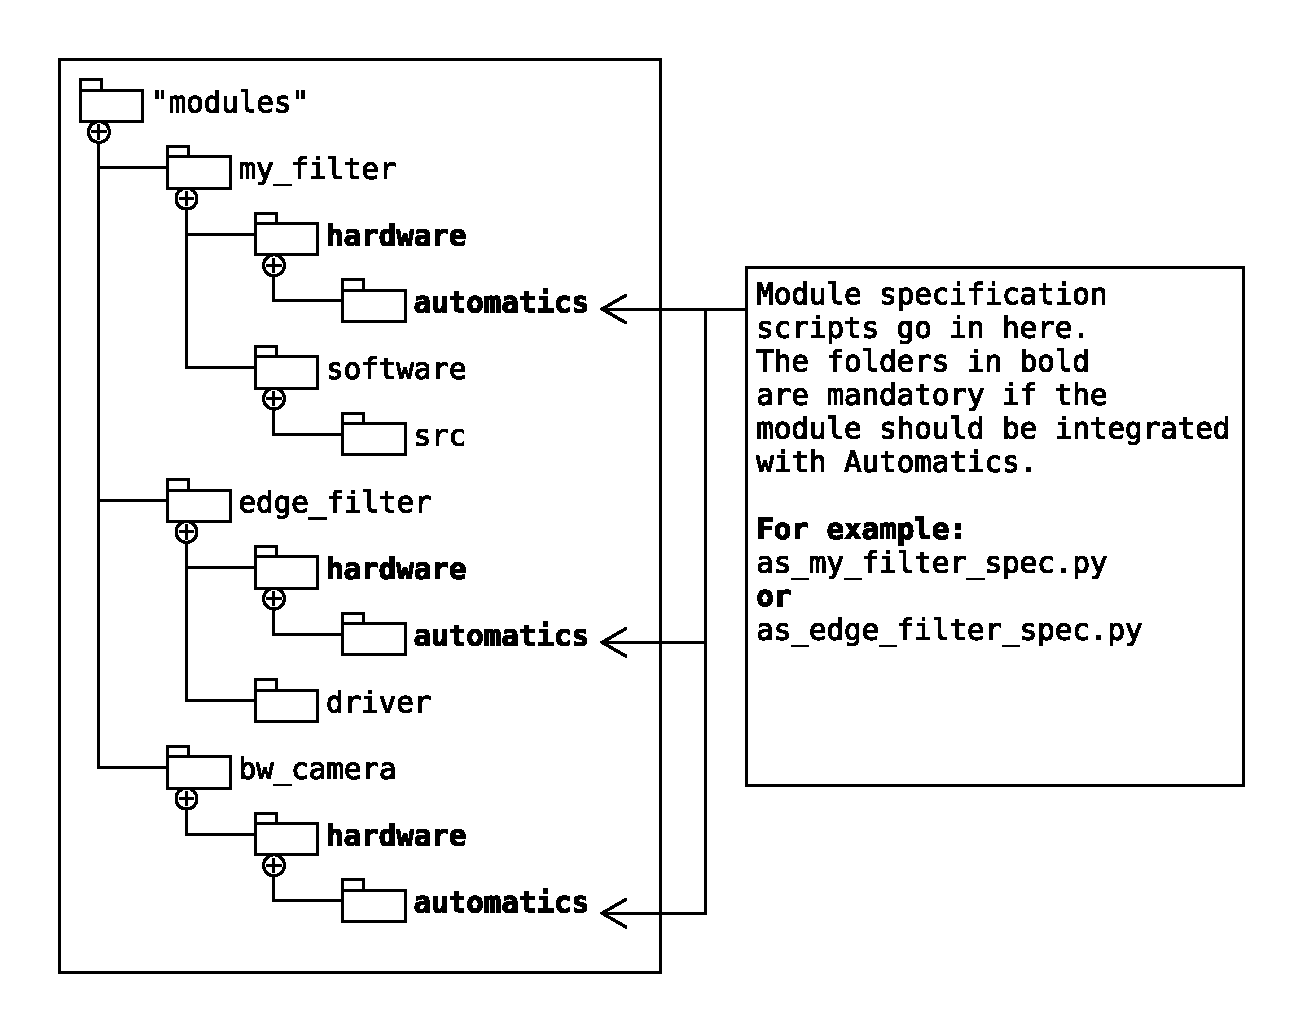
\includegraphics[width=0.9\textwidth]{./figs/06-02-Module_specification_folder_structure.eps}
\caption{Folder structure of source files of modules used with Automatics.}
\label{fig:06-02-module_folder_structure}
\end{figure}

As mentioned in section \ref{ssec:06-02-interface}, in the module specification files before the call to \lstapyinline{module.discover_module} new interface templates may be added to only this module by using the \lstapyinline{module.add_local_interface_template()} method.

Most other configuration options, such as modifying Ports, Generic and Interface settings, must be done after the call to \lstapyinline{module.discover_module()}, as this is the method Automatics uses to create all the Port, Generic and Interface objects.
Refer to the specification template file and the Doxygen documentation or the Python docstrings for explanations of the functionality of the available methods of the different Automatics objects.
Of main interest are the classes Port, Generic, Interface, AsModule, AsWindowModule, WindowInterface, Constant, AsRegisterInterface and AsModuleGroup.

To quickly get started with a custom module, one of the modules included with \asterics, contained in \texttt{asterics/modules} may be used as a starting point.

\subsubsection{Modules for Use in 2D Window Pipeline Systems - Window Modules}
\label{sec:06-02-custom_window_modules}

For modules that can be used in 2D Window Pipeline systems, certain special requisites must be fulfilled.
Firstly, to be correctly connected automatically, the module must be defined for Automatics, as an AsWindowModule Python class.
For this, a separate module specification script template is provided in the directory of all source files of Automatics (\lsthdlinline{asterics/tools/as-automatics/as_automatics_window_module_spec_template.py}).
Here is an example specification script of a window module (\texttt{as\_2d\_conv\_filter\_internal}):
\begin{lstlisting}[style=AutomaticsPython, label=lst:06-02_window_module_spec, caption=Specification script for a typical window module]
from as_automatics_2d_window_module import AsWindowModule

def get_module_instance(module_dir: str) -> AsWindowModule:

    module = AsWindowModule()
    toplevel_file = "hardware/hdl/vhdl/as_2d_conv_filter_internal.vhd"
    module.files = []
    module.dependencies = ["as_generic_filter_module"]
    module.processing_delay = 2

    # Automatics automatically parses the toplevel file and discovers
    # ports, generics, existing interfaces and register interfaces
    module.discover_module(module_dir + "/" + toplevel_file)

    return module
\end{lstlisting}

The only major differences to a regular specification script are first, instead of creating an AsModule object, an AsWindowModule object is created and, with that, all references to AsModule are replaced with AsWindowModule.
Secondly, the additional attribute \lstapyinline{processing\_delay} is set in line 9.
This attribute defines the processing delay in pixels for the module.
A processing delay of zero means that the result for an input is available in the same clock cycle as it was input into the module.
A processing delay of two means that two additional clock cycles are required by the module to process the value and that it will be available after two clock cycles on the modules output.
This value basically describes the number of register stages between the data input and output of the module.
Note that Automatics assumes that all outputs of a module have the same processing delay.
The default value for window modules is one.

Providing this additional meta data along with the same meta data as for a regular AsModule and instantiating it as an AsWindowModule are the only requisites to use a module in 2D Window Pipeline systems.\\

\emph{Note:} Modules declared as AsWindowModules are not usable in regular streaming type chains - only within an As2DWindowPipeline environment - as different connection rules apply. If you would like to use the same module in both contexts, you need to provide two separate specification scripts.
These must be analysed by Automatics either in two separate module repositories to differentiate between modules with identical entity names or point to two separate VHDL source files with different entity names.

\subsubsection{VHDL Coding Rules for \asterics Modules for Use with Automatics}
\label{sec:06-02-vhdl_quirks}

This section lists a few rules that must be followed in VHDL code for Automatics to correctly import a processing module.
These result from quirks of the VHDL Reader used in Automatics to parse the VHDL code.

\begin{itemize}
\item To end a VHDL \lsthdlinline{entity} either the entity name or the keyword \lsthdlinline{entity} must be used after the \lsthdlinline{end} keyword. Eg.: For \lsthdlinline{entity example is [...]} either \lsthdlinline{end example;}, \lsthdlinline{end entity;} or \lsthdlinline{end entity example;} must be used.
\item \lsthdlinline{port} and \lsthdlinline{generic} definitions in an \lsthdlinline{entity} must be in a single line.
\item The beginning and end of both \lsthdlinline{entity} and \lsthdlinline{architecture} must each be in a single line.
\item Port and generic names must not contain any of the following keywords: \lsthdlinline{entity, architecture} and \lsthdlinline{begin}.
\item Port and entity names should be kept all lower-case (within Automatics, they are handled and imported as all lower-case).
\item Generic names should be kept all upper-case (within Automatics, they are handled and imported as all upper-case).
\item The constant for the slave register configuration must be defined and contain the assignment operator (\lsthdlinline{:=}) in a single line. Further value assignments of the array may be spread out onto multiple lines.
\item Further, the constant must be placed before \emph{any} \lsthdlinline{begin} keyword, including \lsthdlinline{begin} as it appears in component, function or procedure declarations.
\end{itemize}

\emph{Note:} Automatics considers only the first entity in each VHDL file as an \asterics module.

All VHDL code after the \lsthdlinline{begin} statement in the \lsthdlinline{architecture} is ignored by Automatics.
No special considerations have to be followed for that code.

\subsubsection{VHDL Coding Rules for AsWindowModules}

For window inputs, VHDL ports that are the input for two dimensional matrices of pixels for filters, a special data type has to be used to facilitate automatic connection using Automatics:
\lsthdlinline{t_generic_window(0 to X, 0 to Y, bit width downto 0)}\\
A second type exists for working with lines of pixels of windows, which works in much the same way:
\lsthdlinline{t_generic_line(0 to X, bit width downto 0)}\\
These data types are specified in the \asterics VHDL package \texttt{as\_generic\_filter}, which must be included when using any of these types.

The range directions (to and downto) for these types \emph{must} be used as described here, as well as the each of the ranges defined meanings.\\

\lsthdlinline{t_generic_window} is the data type used to transfer 2D matrices of pixel data in a compact manner in \asterics.
The first dimension defines the width of the window, the X dimension.
The second dimension defines the height of the window, the Y dimension.
The third dimension defines the data width of the pixels in bits.
The following is an example definition of a 3 by 3 filter window for 8 bit data as a VHDL signal:
\lsthdlinline{signal window : t_generic_window(0 to 2, 0 to 2, 7 downto 0);}\\

\lsthdlinline{t_generic_line} is the data type used to handle single rows of pixel data (pixel arrays) in a manner compatible with \lsthdlinline{t_generic_window} in \asterics.
The first dimension defines the width of the line / row / array.
The second dimension defines the data width of the pixels in bits.
The following is an example definition of a line of 5 pixels with 9 bits each as a VHDL signal:
\lsthdlinline{signal line : t_generic_line(0 to 4, 8 downto 0);}\\

\lsthdlinline{t_integer_array} is a simple unbounded array of integers, used in the function \lsthdlinline{f_make_generic_window}.
It can be used to define fixed filter kernels for use in window modules and can be instantiated as in the following example:
\lsthdlinline{constant filter_values : t_integer_array(0 to 8) := (1,2,1,2,4,2,1,2,1);}\\
Alternatively, the type \lsthdlinline{t_generic_filter} may be used, which is a two dimensional integer array:\\
\lsthdlinline{constant filter_values : t_generic_filter(0 to 2, 0 to 2) := ((1,2,1),(2,4,2),(1,2,1));}



To make working with these data types easier, a number of helper functions are included in the package \texttt{as\_generic\_filter}.
The following is a brief list of all helper functions included for these special data types:
\begin{itemize}
\item \lsthdlinline{f_get_filter_sum_abs(gfilter)}: Calculate and return the absolute sum of all elements of \lsthdlinline{gfilter}.
\item \lsthdlinline{f_get_filter_max(gfilter)}: Find and return the largest value within \lsthdlinline{gfilter}.
\item \lsthdlinline{f_get_filter_elements_count(gfilter)}: Count and return the number of elements of \lsthdlinline{gfilter}.
\item \lsthdlinline{f_get_line_of_generic_filter(gfilter, y)}: Return a \lsthdlinline{t_integer_array} signal equal to the row at index \lsthdlinline{y} of \lsthdlinline{gfilter}.
\item \lsthdlinline{f_get_window_sum_abs(gwindow)}: Calculate and return the absolute sum of all elements of \lsthdlinline{gwindow}.
\item \lsthdlinline{f_get_vector_of_generic_window(gwindow, x, y)}: Extract and return the value of \lsthdlinline{gwindow} at the position (\lsthdlinline{x, y}) as a \lsthdlinline{std_logic_vector}.
\item \lsthdlinline{f_set_vector_of_generic_window(gwindow, x, y, vector)}: Set the value of \lsthdlinline{gwindow} at the position (\lsthdlinline{x, y}) to \lsthdlinline{vector}. Note: \lsthdlinline{vector} must have the same data width as the third dimension of \lsthdlinline{gwindow}!
\item \lsthdlinline{f_get_vector_of_generic_line(gline, x)}: Extract and return the value of \lsthdlinline{gline} at the position(\lsthdlinline{x}) as a \lsthdlinline{std_logic_vector}.
\item \lsthdlinline{f_set_vector_of_generic_line(gline, x, vector)}:  Set the value of \lsthdlinline{gline} at the position (\lsthdlinline{x}) to \lsthdlinline{vector}. Note: \lsthdlinline{vector} must have the same data width as the second dimension of \lsthdlinline{gline}!
\item \lsthdlinline{f_make_generic_window(x, y, values, data_width)}: Create and return a \lsthdlinline{t_generic_window} with the dimensions (\lsthdlinline{x, y, data_width}) and the contents of the \lsthdlinline{t_integer_array values}. Implemented for testing purposes but also useful for the definition of VHDL constants.
\item \lsthdlinline{f_get_line_of_generic_window(gwindow, y)}: Extract and return the row at position (\lsthdlinline{y}) of \lsthdlinline{gwindow} as a \lsthdlinline{t_generic_line} data type.
\item \lsthdlinline{f_set_line_of_generic_window(gwindow, y, line_in)}: Set the value of an entire or part of the row at position (\lsthdlinline{y}) of \lsthdlinline{gwindow} to the contents of \lsthdlinline{line_in}.
\item \lsthdlinline{f_get_part_line_of_generic_window(gwindow, y, from_x, width_part)}:  Extract and return part of the row at position (\lsthdlinline{y}) from position (\lsthdlinline{x}) and with a width of \lsthdlinline{width_part} data values from \lsthdlinline{gwindow} as a \lsthdlinline{t_generic_line} data type.
\item \lsthdlinline{f_cut_vectors_of_generic_line(gline, from_b, width_b)}: Return a \lsthdlinline{t_generic_line} signal based on part of the data of \lsthdlinline{gline} by cutting each data value from  bit \lsthdlinline{from_b} and only including the next \lsthdlinline{width_b} bits.
\item \lsthdlinline{f_cut_vectors_of_generic_window(gwindow, from_b, width_b)}: Return a \lsthdlinline{t_generic_window} signal based on part of the data of \lsthdlinline{gwindow} by cutting each data value from  bit \lsthdlinline{from_b} and only including the next \lsthdlinline{width_b} bits.
\end{itemize}

\subsubsection{Advanced Configuration of Custom Modules}
\label{sec:06-02-advanced_spec_scripts}

As every AsModule is at its core a Python object, they can be infinitely extended by adding methods and attributes in the specification script.
For example the module \texttt{as\_sensor\_ov7670} uses the specification script to add methods configuring the IIC masters that different modules in a system use.
For reference, the file can be found in \lsthdlinline{asterics/modules/as_sensor_ov7670/hardware/automatics/as_sensor_ov7670_spec.py}.
Note that this is an advanced configuration and should only be attempted if you are familiar with Python.
Attributes and methods configured as such will generally not be available in auto-completion features in IDEs and will not be listed for an AsModule when using the interactive modes of Automatics.


Furthermore, for a specific feature of Automatics, auto-instantiating modules, see the attribute \lstapyinline{instantiate_in_top} in section \ref{ssec:06-02-interface}, the method \lstapyinline{auto_inst_config} is defined as \lstapyinline{None} for every module.
It can be overwritten in the specification script to define actions to automatically take when the module is added to the system, as, at that point in the connection process, more information on the makeup of the system is available.
The method will always be passed the module instance itself and a reference to the module that instantiated it.
To see an example of this method being used, see the specification script of the \texttt{as\_regmgr} module in \lsthdlinline{asterics/modules/as_misc/hardware/automatics/as_regmgr_spec.py}.


\subsubsection{Adding a New Interface Template}
\label{sec:06-02-new_interface_template}

This section gives an overview of how interfaces are described in Automatics.

There are two types of interface templates in Automatics.
Both describe the general anatomy of an \lstapyinline{Interface} Automatics class, i.e. the types, directions and names of necessary and optional VHDL ports that comprise the interface.

\begin{itemize}
\item Global interface templates:
These templates are considered every time Automatics analyzes a new module.
This is potentially undesired, especially for interfaces consisting of very few and ports with potentially very generic names, as many false positives can be generated, i.e. interfaces are recognized, where ports are match by coincidence.
Templates are added to the list of global interface templates using the method \lstapyinline{asterics.add_global_interface_template()}.
These are disregarded when the modules that come with \asterics are imported.
Add your template to the file \texttt{as\_automatics\_templates.py} for the template to be considered for all modules imported.

\item Local interface templates:
These templates are only considered when importing a single module and must be added using the method \lstapyinline{module.add_local_interface_template()} within the module's specification script.
\end{itemize}

Each interface template is an abstraction of the Automatics Python class \lstapyinline{Interface}.
To define a new template, you may use the example provided below and modify it to match your interface.

\begin{lstlisting}[style=AutomaticsPython]
from as_automatics_interface import Interface
from as_automatics_port import Port

class AsStream(Interface):
    """Template definition for ASTERICS' 'as_stream' interface."""

    INTERFACE_TYPE_NAME = "as_stream"

    def __init__(self):
        super().__init__(self.INTERFACE_TYPE_NAME)
        self.add_port(Port("strobe"))
        self.add_port(Port("data", data_type="std_logic_vector"))
        self.add_port(Port("data_error", optional=True))
        self.add_port(Port("stall", direction="out", optional=True))
        self.add_port(Port("vsync", optional=True))
        vcomplete = Port("vcomplete", optional=True)
        vcomplete.add_rule("sink_missing", "fallback_port(vsync)", False)
        vcomplete.add_rule(
            "sink_missing", "fallback_port(data_unit_complete)", False
        )
        self.add_port(vcomplete)
        self.add_port(Port("hsync", optional=True))
        hcomplete = Port("hcomplete", optional=True)
        hcomplete.add_rule("sink_missing", "fallback_port(hsync)", False)
        self.add_port(hcomplete)
        self.add_port(Port("data_unit_complete", optional=True))

\end{lstlisting}

We recommend to put your interface templates into a separate file or, if it defined only for a single module, to add it into the specification file for that module.

To define a new template, you need use two classes of Automatics, \lstapyinline{Interface} and \lstapyinline{Port}, lines 1 and 2 import them from their respective Python files.

Line 4 declares a new Python class, in this case named \texttt{AsStream}, that inherits all attributes and functionality of the class \lstapyinline{Interface}.
You may name it (almost) anything you want, though we recommend the name of your interface in PascalCase.

Line 7 defines the name of the interface used by Automatics to refer to it.
Enter the name of your interface type here (must be unique).

Lines 9 and 10 initialize the template class and must be included without modifications.

All lines from line 11 on define the ports that comprise the interface.
You may use the example as guidance but should replace all lines from 11 to 26 with your own definitions.
In this section use the method \lstapyinline{self.add_port()} to add a \lstapyinline{Port} to the template.
Use the constructor \lstapyinline{Port()} to define new ports.

The following parameters can be used to define ports:

\begin{itemize}
\item \texttt{name=""}:
Define the main port name part expected by Automatics to recognize this port.
This means that even if prefixes or suffixes are added to the port name, it is still recognized.
For example: If a port is defined as \texttt{"data"}, Automatics will match the following port names to the port \texttt{"data\_1", "input\_data", "my\_data\_3", "data\_0\_additional"}.
Only if the name fragment \texttt{"data"} is not present, no match occurs.
This parameter must always be provided.
The parameter identifier (\texttt{name}) can be omitted, the first parameter is assumed to be the name of the port.

\item \texttt{direction=""}:
Data direction.
Equal to the VHDL data direction in the entity.
The possible values are: \texttt{"in", "out", "inout"}.
The default value is \texttt{"in"}.
\textit{Note:} The direction \texttt{"inout"} is only supported for external interfaces and ports, meaning interfaces and ports with no connections within the \asterics chain.

\item \texttt{data\_type=""}:
This parameter is equal to the VHDL data type.
No specific limitations exist.
The default value is \texttt{"std\_logic"}.
This parameter is purely treated as a string value and compared to the string extracted from the VHDL entity.

\item \texttt{optional=True/False}:
This boolean value defines whether the Port is necessary for the interface to be considered complete.
If any one port defined as not optional is missing in the entity of a module, that interface is not included in the module.
Inversely, any or all ports defined as optional may be missing in the entity and the interface will still be included.
The default value is \texttt{False}.
\end{itemize}

Furthermore, certain rules can be defined for each port.
To do this, assign a created \lstapyinline{Port} to a temporary variable, as seen with \texttt{vcomplete} in line 16 of the example above.
Now using the variable, the port can be further configured using methods regarding port rules.
A reference of port rule methods can be found in section \ref{sec:06-02-config_methods}.
After configuration, the port must be added to the template using the \lstapyinline{self.add_port()} method, as shown in line 21 of the example.

When using the methods \lstapyinline{asterics.add_global_interface_template()} and \lstapyinline{module.add_local_interface_template()} provide an instance of the template class, for example:
\begin{lstlisting}[style=AutomaticsPython]
# Global template
asterics.add_global_interface_template(AsStream())
# Local template (within module specification)
module.add_local_interface_template(AsStream())
\end{lstlisting}


\subsection{List of Methods for Use in Automatics Scripts}
\label{sec:06-02-config_methods}

This section lists configuration methods intended for use in Automatics scripts of Python classes of Automatics, to configure and build an \asterics processing chain.
All methods of the \lstapyinline{asterics} Python module, also used in Automatics scripts, are listed and detailed in section \ref{sec:06-02-cnns}.
The methods are listed in table \ref{tab:06-02-config_methods}.

A full account of all attributes, functions and methods available in Automatics and its classes can be found in the Doxygen documentation or directly in the source code.

\begin{longtable}[htbp]{|c|c|c|c|}
\hline 
\textbf{Object} & \textbf{Method} & \textbf{Parameters} & \textbf{Description} \\
\hline
\hline
\endhead
% ---------- AsProcessingChain --------------
\parbox{2.5cm}{~\\ \texttt{AsProcessing Chain}\\~} & \parbox{3cm}{~\\ \texttt{add\_module()}\\~} & \parbox{3cm}{~ \\ \texttt{entity\_name , user\_name, repo\_name} \\ ~} & \parbox{6cm}{~\\ Adds the module \texttt{entity\_name} from the module library to the processing chain. Optionally the module can be named using the \texttt{user\_name}, if ommitted, Automatics will enumerate using the \texttt{entity\_name}. Optionally, using the \texttt{repo\_name} a module can be chosen from a specific module repository. Useful to differentiate between modules with the same entity name imported from different repositories. \\~}\\
\hline
\parbox{2.5cm}{~\\ \texttt{AsProcessing Chain}\\~} & \parbox{3cm}{~\\ \texttt{set\_asterics\\\_base\_address()}\\~} & \parbox{3cm}{~ \\ \texttt{base\_address, address\_ space\_size} \\ ~} & \parbox{6cm}{~\\ Redefine the \asterics base address for communication between the \asterics modules and software. Set the available address space. \emph{Important:} Note that the base address must begin with all bits in the available space as zero. Eg.: OK: Base = \texttt{0x43C10000} and Size = \texttt{0xFFFF}, not OK: Base = \texttt{0x43C18000} and Size = \texttt{0x8FFF} (must be Base = \texttt{0x43C1{\color{blue}0}000}) \\~}\\
\hline
\parbox{2.5cm}{~\\ \texttt{AsProcessing Chain}\\~} & \parbox{3cm}{~\\ \texttt{connect()}\\~} & \parbox{3cm}{~ \\ \texttt{from, to} \\ ~} & \parbox{6cm}{~\\ Connect module, interface or port \texttt{from} to module, interface or port \texttt{to}. The direction of data flow is assumed to be from \texttt{from} to \texttt{to}, though an internal inspection will swap the objects if necessary. Note: The method call will be forwarded to the connect method of As2DWindowPipeline, if any object is part of a pipeline. \\~}\\
\hline
\parbox{2.5cm}{~\\ \texttt{AsProcessing Chain}\\~} & \parbox{3cm}{~\\ \texttt{write\_hw()}\\~} & \parbox{3cm}{~ \\ \texttt{folder, use\_symlinks, force} \\ ~} & \parbox{6cm}{~\\ Generate only the hardware source output files to \texttt{folder}. By default existing module source files are linked to the output folder. To copy them instead, use \lstapyinline{use_symlinks=False}. To allow Automatics to clean the output folder by permanently deleting contained files, set \lstapyinline{force=True}. \\~}\\
\hline
\parbox{2.5cm}{~\\ \texttt{AsProcessing Chain}\\~} & \parbox{3cm}{~\\ \texttt{write\_sw()}\\~} & \parbox{3cm}{~ \\ \texttt{folder, use\_symlinks, force, driver\_module\_\\\_dirs} \\ ~} & \parbox{6cm}{~\\ Generate only the software source output files to \textit{folder}. By default existing module source files are linked to the output folder. To copy them instead, use \lstapyinline{use_symlinks=False}.  To allow Automatics to clean the output folder by permanently deleting contained files, set \textit{force=True}. If you want source files sorted into subfolders per module, set \lstapyinline{driver_module_dirs=True}. \\~}\\
\hline
\parbox{2.5cm}{~\\ \texttt{AsProcessing Chain}\\~} & \parbox{3cm}{~\\ \texttt{write\_asterics\_\\ \_core()}\\~} & \parbox{3cm}{~ \\ \texttt{folder, use\_symlinks, force, driver\_module\_\\\_dirs} \\ ~} & \parbox{6cm}{~\\ Runs both \lstapyinline{write_hw()} and \lstapyinline{write_sw()}. The parameters are identical in functionality to those methods. \\~}\\
\hline
\parbox{2.5cm}{~\\ \texttt{AsProcessing Chain}\\~} & \parbox{3cm}{~\\ \texttt{write\_ip\_core\_\\ \_xilinx()}\\~} & \parbox{3cm}{~ \\ \texttt{folder, use\_symlinks, force, driver\_module\_ dirs} \\ ~} & \parbox{6cm}{~\\ Runs both \lstapyinline{write_hw()} and \lstapyinline{write_sw()}. The parameters are identical in functionality to those methods. In addition, the resulting IP-Core is packaged using Vivado. Vivado has to be installed on your system and sourced in the console environment you used to run Automatics for this step to complete. \\~}\\
\hline
\parbox{2.5cm}{~\\ \texttt{AsProcessing Chain}\\~} & \parbox{3cm}{~\\ \texttt{write\_system()}\\~} & \parbox{3cm}{~ \\ \texttt{folder, use\_symlinks, force, driver\_module\_\\\_dirs, add\_vears} \\ ~} & \parbox{6cm}{~\\ Runs both \lstapyinline{write_hw()} and \lstapyinline{write_sw()}. The parameters are identical in functionality to those methods.
The outputs are generated into a system template prepared for a Vivado-style FPGA project. In addition, the resulting IP-Core is packaged using Vivado. Vivado has to be installed on the system and sourced in the console environment used to run Automatics for this step to complete. Furthermore, the VEARS IP-Core for video output is added to the project. To omit it, set \lstapyinline{add_vears=False}. \\~}\\
\hline
\parbox{2.5cm}{~\\ \texttt{AsProcessing Chain}\\~} & \parbox{3cm}{~\\ \texttt{write\_system\_ graph()}\\~} & \parbox{3cm}{~ \\ \texttt{out\_file, show\_ toplevels, show\_auto\_ inst, show\_ports} \\ ~} & \parbox{6cm}{~\\ Generate and write a graph representation of the system represented by chain to the file \texttt{out\_file}. The other parameters are all \lstapyinline{False} by default and may be turned on (\lstapyinline{True}) to add detail. \texttt{show\_toplevels} adds "meta modules" used to connect  processing modules. \texttt{show\_auto\_inst} adds automatically instantiated modules. \texttt{show\_ports} adds a list of all ports to each edge of the graph which represent interfaces. \\~}\\
\hline
\parbox{2.5cm}{~\\ \texttt{AsProcessing Chain}\\~} & \parbox{3cm}{~\\ \texttt{list\_address \_space()}\\~} & \parbox{3cm}{~ \\ \texttt{None} \\ ~} & \parbox{6cm}{~\\ Call after building the processing chain to list the addresses and types of all allocated slave registers of the included modules. \\~}\\
\hline


% ---------- AsNNLayer --------------

\parbox{2.5cm}{~\\ \texttt{AsNNLayer}\\~} & \parbox{3cm}{~\\ \texttt{parametrize\_ and\_build()}\\~} & \parbox{3cm}{~ \\ \texttt{- omitted for brevity -} \\ ~} & \parbox{6cm}{~\\ Configure the neural network layer subsystem. The parameters are explained in section \ref{ssec:06-02-cnn_accel_module}.  \\~}\\
\hline

% ---------- As2DWindowPipeline --------------

\parbox{2.5cm}{~\\ \texttt{As2DWindow Pipeline}\\~} & \parbox{3cm}{~\\ \texttt{add\_module()}\\~} & \parbox{3cm}{~ \\ \texttt{entity\_name, user\_name, repo\_name} \\ ~} & \parbox{6cm}{~\\ Add a module to this As2DWindowPipeline with the entity name \texttt{entity\_name}. \emph{Only window modules} are considered when selecting the module. Optionally a name can be set for the module using \texttt{user\_name}. Optionally, using the \texttt{repo\_name} a module can be chosen from a specific module repository. Useful to differentiate between modules with the same entity name imported from different repositories.  \\~}\\
\hline
\parbox{2.5cm}{~\\ \texttt{As2DWindow Pipeline}\\~} & \parbox{3cm}{~\\ \texttt{connect()}\\~} & \parbox{3cm}{~ \\ \texttt{from, to, no\_delay, no\_stall} \\ ~} & \parbox{6cm}{~\\ Connect two objects, \texttt{from} and \texttt{to}, with each other within the pipeline. Additional optional parameters: \texttt{no\_delay}: if \texttt{from} is outside of the pipeline and this parameter is set to \lstapyinline{True}, no buffers to synchronize this input with all other input data will be created. \texttt{no\_stall}: if \texttt{to} is an \texttt{as\_stream} interface outside of the pipeline and \texttt{no\_stall} is set to \lstapyinline{True}, the \texttt{stall} signal of the target \texttt{as\_stream} interface will not be connected. Note: Calls to the processing chain's connect method with objects of a pipeline, will be forwarded to the pipeline's connect method, allowing for \lstapyinline{module0.connect(module1)} calls to connect modules of a pipeline.\\~}\\
\hline
\parbox{2.5cm}{~\\ \texttt{As2DWindow Pipeline}\\~} & \parbox{3cm}{~\\ \texttt{set\_flushing\_ behaviour()}\\~} & \parbox{3cm}{~ \\ \texttt{debug\_ flushdata, constant\_ flushdata\_ value} \\ ~} & \parbox{6cm}{~\\ Configure the behaviour of the flush control module included with every pipeline. Use \texttt{debug\_flushdata} to use a pixel counter as the flush data (\lstapyinline{True}) or a constant data word as flush data (\texttt{False}, default). Use \texttt{constant\_flushdata\_value} to define a custom value for the constant flush data. Default: 128. \\~}\\
\hline
\parbox{2.5cm}{~\\ \texttt{As2DWindow Pipeline}\\~} & \parbox{3cm}{~\\ \texttt{set\_main\_ buffer\_ optimization\_ strategy()}\\~} & \parbox{3cm}{~ \\ \texttt{new\_strategy} \\ ~} & \parbox{6cm}{~\\ Set the optimization strategy to use when optimizing the buffers of the window ports of the pipeline. Available optimizations are attributes of the pipeline object and prefixed with \lstapyinline{optimize\_}. Available options are: \lstapyinline{optimize\_none}, \lstapyinline{optimize\_row\_number\_sensitive}, \lstapyinline{optimize\_window\_width\_sensitive} and \lstapyinline{optimize\_all\_same\_length}; For a detailed explanation of the effects of each strategy, refer to section \ref{sec:06-02-2dpipe_general}\\~}\\
\hline
\parbox{2.5cm}{~\\ \texttt{As2DWindow Pipeline}\\~} & \parbox{3cm}{~\\ \texttt{set\_similar\_ length\_ optimization()}\\~} & \parbox{3cm}{~ \\ \texttt{active, max\_length\_ difference} \\ ~} & \parbox{6cm}{~\\ Configure the \textit{similar\_length} optimization step. Use \texttt{active} to turn the optimization on (\lstapyinline{True} (default)) and off (\lstapyinline{False}). Use \texttt{max\_length\_difference} to define the maximum length in pixels that buffers are merged. Higher numbers will result in less block-RAM tile usage but higher slice register usage (default: 100). \\~}\\
\hline
\parbox{2.5cm}{~\\ \texttt{As2DWindow Pipeline}\\~} & \parbox{3cm}{~\\ \texttt{set\_reshape\_ long\_buffers\_ optimization()}\\~} & \parbox{3cm}{~ \\ \texttt{active, minimum\_length \_to\_reshape, maximum\_width\_ to\_reshape} \\ ~} & \parbox{6cm}{~\\ Configure the \textit{reshape\_long\_buffers} optimization step. Use \texttt{active} to turn the optimization on (\lstapyinline{True} (default)) and off (\lstapyinline{False}). Use \texttt{minimum\_length\_to\_reshape} to define the minimum buffer length to be reshaped. With default value (-1) a value will be calculated from the pipeline's attribute \texttt{minimum\_bram\_size}. Use \texttt{maximum\_width\_to\_reshape} to define a maximum bit width of buffers to reshape. For additional details about the effects of this optimization, refer to section \ref{sec:06-02-2dpipe_general}. \\~}\\
\hline
\parbox{2.5cm}{~\\ \texttt{As2DWindow Pipeline}\\~} & \parbox{3cm}{~\\ \texttt{print\_pipeline\_ buffer\_report()}\\~} & \parbox{3cm}{~ \\ \texttt{verbosity} \\ ~} & \parbox{6cm}{~\\ Print a summary report of the buffer usage of the pipeline. Set \texttt{verbosity} to 1 to also print a report for every buffer. \\~}\\
\hline
% ---------- AsModuleGroup --------------

\parbox{2.5cm}{~\\ \texttt{AsModule Group} \\ and\\ \texttt{As2DWindow Pipeline}\\~} & \parbox{3cm}{~\\ \texttt{add\_register()}\\~} & \parbox{3cm}{~ \\ \texttt{register\_ type} \\ ~} & \parbox{6cm}{~\\ Create a 32 bit slave register for this module group. Use \texttt{register\_type} to define the type of register. Use \lstapyinline{asterics.Register.<type>} for the parameter. Possible types are \lstapyinline{none, control, status, both}. Refer to section \ref{sec:05-01-05-register_interface} for explanations on the different register types. \\~}\\
\hline
\parbox{2.5cm}{~\\ \texttt{AsModule Group} \\ and\\ \texttt{As2DWindow Pipeline}\\~} & \parbox{3cm}{~\\ \texttt{modify\_ register\_ type()}\\~} & \parbox{3cm}{~ \\ \texttt{register\_num, new\_type} \\ ~} & \parbox{6cm}{~\\ Modify the register type of the register with index \texttt{register\_num} to the type \texttt{new\_type}. For the value of \texttt{new\_type} use the same values as for the method \lstapyinline{add\_register} above. \\~}\\
\hline
\parbox{2.5cm}{~\\ \texttt{AsModule Group} \\ and\\ \texttt{As2DWindow Pipeline}\\~} & \parbox{3cm}{~\\ \texttt{assign\_ register\_ to\_port()}\\~} & \parbox{3cm}{~ \\ \texttt{register\_num, port, from\_bit\_ index} \\ ~} & \parbox{6cm}{~\\ Assign the value, or part of the value of a 32 bit slave register with index \texttt{register\_num} to the port or signal \texttt{port}. The port or signal will be assigned from the registers bit index \texttt{from\_bit\_index} up to the signals or ports bit width. The register will be automatically created if it doesn't exist. \\~}\\
\hline
\parbox{2.5cm}{~\\ \texttt{AsModule Group} \\ and\\ \texttt{As2DWindow Pipeline}\\~} & \parbox{3cm}{~\\ \texttt{assign\_port\_ to\_register()}\\~} & \parbox{3cm}{~ \\ \texttt{register\_num, port, to\_bit\_ index} \\ ~} & \parbox{6cm}{~\\ Assign the value of the port or signal \texttt{port} to a 32 bit slave register with index \texttt{register\_num}. The port or signals value will be assigned from the registers bit index \texttt{to\_bit\_index} up to the ports or signals bit width. The register will be automatically created if it doesn't exist. \\~}\\
\hline
\parbox{2.5cm}{~\\ \texttt{AsModule Group} \\ and\\ \texttt{As2DWindow Pipeline}\\~} & \parbox{3cm}{~\\ \texttt{define\_port()}\\~} & \parbox{3cm}{~ \\ \texttt{name, code\_name, direction, data\_type, data\_width, fixed\_value} \\ ~} & \parbox{6cm}{~\\ Create, add and return a new Port object for this module group. \texttt{name} defines the base name of the new Port. The optional \texttt{code\_name} defines the name of the port in VHDL, default is the value of \texttt{name}. The optional \texttt{direction} defines the data direction of the port. Valid values are \lstapyinline{"in"} (default), \lstapyinline{"out"} and \lstapyinline{"inout"} (only partial support for automatic connections). The optional \texttt{data\_type} defines the VHDL data type of the port. Default: \lsthdlinline{std\_logic}. The optional \texttt{"data\_width"} defines the data width for vector types. Use a Python tuple, e. g. \lstapyinline{(0, "to", 7)} or \lstapyinline{"DATA_WIDTH - 1", "downto", 0)}. Anything but single numbers must be passed as a string. The optional \texttt{fixed\_value} can be used to define a fixed value for the port as a string. Only useful for ports with direction \lstapyinline{"out"}. Note that ports with a fixed value have a limited support for connections, as they will be assigned the fixed value within the module group. \\~}\\
\hline
\parbox{2.5cm}{~\\ \texttt{AsModule Group} \\ and\\ \texttt{As2DWindow Pipeline}\\~} & \parbox{3cm}{~\\ \texttt{define\_signal()}\\~} & \parbox{3cm}{~ \\ \texttt{name, data\_type, data\_width, fixed\_value} \\ ~} & \parbox{6cm}{~\\ Create, add and return a new GenericSignal object for this module group. The parameters work analogous to the method \texttt{define\_port} above, with following exceptions: The \texttt{name} will always be used as the \texttt{code\_name} attribute of the signal. The \texttt{fixed\_value} is more useful as signals do not have a data direction and exist only within a module group. \\~}\\
\hline

% ---------- AsModule --------------

\parbox{2.5cm}{~\\ \texttt{AsModule}\\~} & \parbox{3cm}{~\\ \texttt{add\_software\_ driver\_file()}\\~} & \parbox{3cm}{~ \\ \texttt{path} \\ ~} & \parbox{6cm}{~\\ Add an additional software driver file to this module. The path may be relative from the execution location of the chain description script or absolute. \\~}\\
\hline
\parbox{2.5cm}{~\\ \texttt{AsModule}\\~} & \parbox{3cm}{~\\ \texttt{connect()}\\~} & \parbox{3cm}{~ \\ \texttt{object} \\ ~} & \parbox{6cm}{~\\ Shorthand for \lstapyinline{chain.connect(self, object)}. Can also be used for modules that are part of a 2D Window Pipeline. \\~}\\
\hline
\parbox{2.5cm}{~\\ \texttt{AsModule}\\~} & \parbox{3cm}{~\\ \texttt{get\_port()}\\~} & \parbox{3cm}{~ \\ \texttt{port\_name} \\ ~} & \parbox{6cm}{~\\ Return the Port of the module with the \texttt{code\_name} or \texttt{name} attribute \texttt{port name}. \\~}\\
\hline
\parbox{2.5cm}{~\\ \texttt{AsModule}\\~} & \parbox{3cm}{~\\ \texttt{get\_interface()}\\~} & \parbox{3cm}{~ \\ \texttt{interface\_name, direction, interface\_type} \\ ~} & \parbox{6cm}{~\\ Return the Interface of the module with the \texttt{name} and \texttt{pre-/suffix} attributes matching \texttt{interface\_name}. Optionally exclude any interfaces from the search not matching with \texttt{direction} and/or \texttt{interface\_type}. \\~}\\
\hline
\parbox{2.5cm}{~\\ \texttt{AsModule}\\~} & \parbox{3cm}{~\\ \texttt{get()}\\~} & \parbox{3cm}{~ \\ \texttt{name, direction} \\ ~} & \parbox{6cm}{~\\ Shorthand for a combination of \lstapyinline{get\_interface} and \lstapyinline{get\_port}. Returns the first interface matching \texttt{name} and \texttt{direction} or, if none was found, searches for a matching port instead.\\~}\\
\hline
\parbox{2.5cm}{~\\ \texttt{AsModule}\\~} & \parbox{3cm}{~\\ \texttt{get\_generic()}\\~} & \parbox{3cm}{~ \\ \texttt{generic\_name} \\ ~} & \parbox{6cm}{~\\ Return the Generic of the module with the \texttt{code\_name} or \texttt{name} attribute \texttt{generic\_name}. \\~}\\
\hline
\parbox{2.5cm}{~\\ \texttt{AsModule}\\~} & \parbox{3cm}{~\\ \texttt{make\_port \_external()}\\~} & \parbox{3cm}{~ \\ \texttt{port\_name, value} \\ ~} & \parbox{6cm}{~\\ Search for a Port matching \texttt{port\_name} and change it's \texttt{ruleset} to have Automatics make it external (default), meaning it will be available on the interface of the resulting IP-Core. Alternatively, make an external port internal by setting \texttt{value} to \lstapyinline{False}. \\~}\\
\hline
\parbox{2.5cm}{~\\ \texttt{AsModule}\\~} & \parbox{3cm}{~\\ \texttt{make\_interface \_external()}\\~} & \parbox{3cm}{~ \\ \texttt{interface\_name, direction, if\_type, value} \\ ~} & \parbox{6cm}{~\\ Search for an Interface matching \texttt{interface\_name} (and optionally \texttt{direction} and \texttt{if\_type}) to have Automatics make it external (default: \texttt{value} set to \lstapyinline{True}), meaning it will be available on the interface of the resulting IP-Core. Alternatively, make an external interface internal by setting \texttt{value} to \lstapyinline{False}. Note that you will have to either provide the parameter name (\lstapyinline{value=False}) or use all parameters. \\~}\\
\hline

\parbox{2.5cm}{~\\ \texttt{AsModule}\\~} & \parbox{3cm}{~\\ \texttt{set\_port \_fixed\_value()}\\~} & \parbox{3cm}{~ \\ \texttt{port\_name, value} \\ ~} & \parbox{6cm}{~\\ Search for a Port matching \texttt{port\_name} and change it's \texttt{ruleset} to have Automatics set it to the fixed value \texttt{value}. Automatics will directly insert the value of \texttt{value} into VHDL code, therefore it must adhere to VHDL syntax. \\~}\\
\hline
\parbox{2.5cm}{~\\ \texttt{AsModule}\\~} & \parbox{3cm}{~\\ \texttt{set\_generic \_value()}\\~} & \parbox{3cm}{~ \\ \texttt{generic\_name, value} \\ ~} & \parbox{6cm}{~\\ Search for a Generic of the module with the name \texttt{generic\_name} and set it's \texttt{value} attribute to the value of the parameter \texttt{value}. Note that the value of \texttt{value} will be directly inserted into VHDL code, therefore it must adhere to VHDL syntax. \\~}\\
\hline
\parbox{2.5cm}{~\\ \texttt{AsModule}\\~} & \parbox{3cm}{~\\ \texttt{port\_rule \_add()}\\~} & \parbox{3cm}{~ \\ \texttt{port\_name, condition, action, priority} \\ ~} & \parbox{6cm}{~\\ Search for a Port matching \texttt{port\_name} and add to it's \texttt{ruleset} the new rule \texttt{condition -> action}. This rule will have top priority, so will be executed first, unless the parameter \texttt{priority} is set to \lstapyinline{False}. \\~}\\
\hline
\parbox{2.5cm}{~\\ \texttt{AsModule}\\~} & \parbox{3cm}{~\\ \texttt{port\_rule \_remove()}\\~} & \parbox{3cm}{~ \\ \texttt{port\_name, condition, action} \\ ~} & \parbox{6cm}{~\\ Search for a Port matching \texttt{port\_name} and remove the rule \texttt{condition -> action} from it's \texttt{ruleset}, if it exists. \\~}\\
\hline
\parbox{2.5cm}{~\\ \texttt{AsModule}\\~} & \parbox{3cm}{~\\ \texttt{port\_rule \_overwrite()}\\~} & \parbox{3cm}{~ \\ \texttt{port\_name, condition, action} \\ ~} & \parbox{6cm}{~\\ Search for a Port matching \texttt{port\_name} and overwrite all \texttt{actions} for \texttt{condition} in it's \texttt{ruleset}. Then add the rule \texttt{condition -> action}. \\~}\\
\hline
\parbox{2.5cm}{~\\ \texttt{AsModule}\\~} & \parbox{3cm}{~\\ \texttt{make\_generic \_external()}\\~} & \parbox{3cm}{~ \\ \texttt{generic\_name} \\ ~} & \parbox{6cm}{~\\ For the Generic matching \texttt{generic\_name}, set its attributes so that it will be propagated to toplevel, allowing the synthesis tool to set the value using the \asterics IP-Core.\\~}\\
\hline

% ---------- Interface --------------
\parbox{2.5cm}{~\\ \texttt{Interface}\\~} & \parbox{3cm}{~\\ \texttt{connect()}\\~} & \parbox{3cm}{~ \\ \texttt{object} \\ ~} & \parbox{6cm}{~\\ Shorthand for \lstapyinline{chain.connect(self, object)}. Can also be used for interfaces that are part of modules within a 2D Window Pipeline. \\~}\\
\hline
\parbox{2.5cm}{~\\ \texttt{Interface}\\~} & \parbox{3cm}{~\\ \texttt{make\_external()}\\~} & \parbox{3cm}{~ \\ \texttt{value} \\ ~} & \parbox{6cm}{~\\ Set the necessary attribute to make this Interface available externally. Automatics will connect it to the VHDL toplevel, so it is in the interface of the resulting IP-Core. Set \texttt{value} to \lstapyinline{False} to make external interfaces internal. \\~}\\
\hline
\parbox{2.5cm}{~\\ \texttt{Interface}\\~} & \parbox{3cm}{~\\ \texttt{instantiate \_module()}\\~} & \parbox{3cm}{~ \\ \texttt{entity\_name, group\_name} \\ ~} & \parbox{6cm}{~\\ Set the necessary attributes to have Automatics automatically add and instantiate the \asterics module \texttt{entity\_name} and connect the interface to it. The \texttt{group\_name} defines where in the hardware design the module is instantiated. This particular functionality is currently not implemented completely - the only two options for the \texttt{group\_name} are: \lstapyinline{asterics}, to instantiate to the toplevel (default) and \lstapyinline{as_main} to instantiate the module where the \asterics modules are connected. This functionality is useful, for example, to instantiate necessary bus manager modules or similar. \\~}\\
\hline
\parbox{2.5cm}{~\\ \texttt{Interface}\\~} & \parbox{3cm}{~\\ \texttt{instantiate \_no\_module()}\\~} & \parbox{3cm}{~ \\ \texttt{None} \\ ~} & \parbox{6cm}{~\\ Remove a configuration for an automatic instantiation of a mode from this interface object. \\~}\\
\hline

% ---------- Generic --------------
\parbox{2.5cm}{~\\ \texttt{Generic}\\~} & \parbox{3cm}{~\\ \texttt{link\_to \_generic()}\\~} & \parbox{3cm}{~ \\ \texttt{link\_generic} \\ ~} & \parbox{6cm}{~\\ Set the necessary attributes to have Automatics link the value of this Generic to the Generic \texttt{link\_generic}, using the \texttt{code\_name} attribute, of higher modules. This can be useful, for example, to set the data bus width of multiple modules, using a user added Generic on the toplevel. (Note: This feature has not been tested extensively.) \\~}\\
\hline

% ---------- GenericSignal ----------

\parbox{2.5cm}{~\\ \texttt{Generic Signal}\\~} & \parbox{3cm}{~\\ \texttt{assign\_ from\_this\_ vector()}\\~} & \parbox{3cm}{~ \\ \texttt{target, from\_bit\_ index} \\ ~} & \parbox{6cm}{~\\ Partially assign from this signal. Only applicable for signals with a vector data type. Assign to port or signal \texttt{target} starting with bit index \texttt{from\_bit\_index} of the signal with the width of the target port or signal. \\~}\\
\hline
\parbox{2.5cm}{~\\ \texttt{Generic Signal}\\~} & \parbox{3cm}{~\\ \texttt{assign\_ to\_this\_ vector()}\\~} & \parbox{3cm}{~ \\ \texttt{source, from\_bit\_ index} \\ ~} & \parbox{6cm}{~\\ Assign the port or signal \texttt{source} to part of this signal. Only applicable for signals of a vector data type. Assign the source port or signal starting from bit index \texttt{from\_bit\_index} up to the data width of the source port or signal. \\~}\\
\hline
\parbox{2.5cm}{~\\ \texttt{Generic Signal}\\~} & \parbox{3cm}{~\\ \texttt{define\_ vector\_ assignment()}\\~} & \parbox{3cm}{~ \\ \texttt{source\_ list} \\ ~} & \parbox{6cm}{~\\ Define a list of source ports or signals \texttt{source\_list} to completely define the assignment of this signal. Only applicable for signals with a vector data type. The assignment starts at bit index zero and advances by the data width of each source port or signal in the list. The list keeps its order and will not be sorted. Equates to repeated calls to \lstapyinline{assign\_to\_this\_vector}. \\~}\\
\hline

% ---------- Port --------------
\parbox{2.5cm}{~\\ \texttt{Port} \\ and\\ \texttt{Generic Signal}\\~} & \parbox{3cm}{~\\ \texttt{connect()}\\~} & \parbox{3cm}{~ \\ \texttt{object} \\ ~} & \parbox{6cm}{~\\ Shorthand for \lstapyinline{chain.connect(self, object)}. Can also be used for ports that are part of modules within a 2D Window Pipeline. \\~}\\
\hline
\parbox{2.5cm}{~\\ \texttt{Port} \\ and\\ \texttt{Generic Signal}\\~} & \parbox{3cm}{~\\ \texttt{set\_port \_type()}\\~} & \parbox{3cm}{~ \\ \texttt{port type} \\ ~} & \parbox{6cm}{~\\ Manually define the Port's \texttt{port\_type} attribute. Useful if a Port is determined to have the wrong port type by Automatics. Valid values: \lstapyinline{"single"}, \lstapyinline{"external"}, \lstapyinline{"interface"}, \lstapyinline{"register"}, \lstapyinline{"signal"}, \lstapyinline{"glue\_signal"}. \\~}\\
\hline
\parbox{2.5cm}{~\\ \texttt{Port} \\ and\\ \texttt{Generic Signal}\\~} & \parbox{3cm}{~\\ \texttt{remove \_condition()}\\~} & \parbox{3cm}{~ \\ \texttt{condition} \\ ~} & \parbox{6cm}{~\\ Remove all rules with the condition \texttt{condition} from this Port's \texttt{ruleset}. You may use \lstapyinline{module.port_rule_overwrite}
\lstapyinline{(<port name>, <condition>, "none")} for the same effect. \\~}\\
\hline
\parbox{2.5cm}{~\\ \texttt{Port}\\ and\\ \texttt{Generic Signal}\\~} & \parbox{3cm}{~\\ \texttt{update \_ruleset()}\\~} & \parbox{3cm}{~ \\ \texttt{list} \\ ~} & \parbox{6cm}{~\\ Use this method to quickly add multiple rules to this Port's \texttt{ruleset}. Note that any invalid rules are quietly skipped. Any iterable list is accepted. Note that the rules are expected to use the \lstapyinline{Port.Rule namedtuple} (refer to the file \texttt{as\_automatics\_port.py}). \\~}\\
\hline
\parbox{2.5cm}{~\\ \texttt{Port} \\ and\\ \texttt{Generic Signal}\\~} & \parbox{3cm}{~\\ \texttt{set\_ruleset()}\\~} & \parbox{3cm}{~ \\ \texttt{list} \\ ~} & \parbox{6cm}{~\\ Use this method to quickly replace this Port's \texttt{ruleset}. Note that any invalid rules are quietly skipped. Any iterable list is accepted. Note that the rules are expected to use the \lstapyinline{Port.Rule namedtuple} (refer to the file \texttt{as\_automatics\_port.py}). \\~}\\
\hline

\parbox{2.5cm}{~\\ \texttt{Port} \\ and\\ \texttt{Generic Signal}\\~} & \parbox{3cm}{~\\ \texttt{add\_rule()}\\~} & \parbox{3cm}{~ \\ \texttt{rule\_condition}, \texttt{rule\_action}, \texttt{priority} \\ ~} & \parbox{6cm}{~\\ This method adds a Port rule condition, action pair. If the parameter \lstapyinline{priority} is set to \lstapyinline{True} (default) the new rule is inserted as the first rule to be applied when handling the port, giving it precedence over all prior rules. If \lstapyinline{priority} is set to  \lstapyinline{False} the new rule will be the last one to be applied. Refer to section \ref{ssec:06-02-class_port} for a full account of port rule conditions and actions. \\~}\\
\hline

\parbox{2.5cm}{~\\ \texttt{Port} \\ and\\ \texttt{Generic Signal}\\~} & \parbox{3cm}{~\\ \texttt{overwrite\_\\rule()}\\~} & \parbox{3cm}{~ \\ \texttt{rule\_condition}, \texttt{new\_action} \\ ~} & \parbox{6cm}{~\\ This method removes any rules using the condition \lstapyinline{rule_condition} and inserts the rule defined by \lstapyinline{rule_condition}, \lstapyinline{new_action}.
If no rules with \lstapyinline{rule_condition} exist, the new rule will not be inserted into the ruleset. \\~}\\
\hline

\parbox{2.5cm}{~\\ \texttt{Port} \\ and\\ \texttt{Generic Signal}\\~} & \parbox{3cm}{~\\ \texttt{remove\_rule()}\\~} & \parbox{3cm}{~ \\ \texttt{condition}, \texttt{action} \\ ~} & \parbox{6cm}{~\\ This method removes the first rule defined by both the specified \lstapyinline{condition} and \lstapyinline{action}. \\~}\\
\hline

\parbox{2.5cm}{~\\ \texttt{Port} \\ and\\ \texttt{Generic Signal}\\~} & \parbox{3cm}{~\\ \texttt{remove\_\\condition()}\\~} & \parbox{3cm}{~ \\ \texttt{rule\_condition} \\ ~} & \parbox{6cm}{~\\ This method removes all rules using the specified \lstapyinline{condition} from the port's ruleset. \\~}\\
\hline

\parbox{2.5cm}{~\\ \texttt{Port} \\ and\\ \texttt{Generic Signal}\\~} & \parbox{3cm}{~\\ \texttt{remove\_\\rule\_action()}\\~} & \parbox{3cm}{~ \\ \texttt{rule\_action} \\ ~} & \parbox{6cm}{~\\ This method removes all rules using the specified \lstapyinline{rule_action} from the port's ruleset. \\~}\\
\hline

\parbox{2.5cm}{~\\ \texttt{Port} \\~} & \parbox{3cm}{~\\ \texttt{make \_external()}\\~} & \parbox{3cm}{~ \\ \texttt{None} \\ ~} & \parbox{6cm}{~\\ Modify this Port's \texttt{ruleset} to have Automatics make it external. Same as AsModule's \lstapyinline{make_port_external()} method. \\~}\\
\hline

\caption{List of configuration methods intended for use in the user script.}
\label{tab:06-02-config_methods}
\end{longtable}





